\section{Rings and Modules of Fractions}
The formation of rings of fractions and the associated process of localization are perhaps the most important technical tools in commutative algebra. They correspond in the algebro-geometric picture to concentrating attention on an open set or near a point, and the importance of these notions should be self-evident. This section gives the definitions and simple properties of the formation of fractions.
\subsection{Basic Concepts}
In this section we shall sketch a brief review of the fraction of a ring. Most results presented here have been introduced in Section 4.4.\par
Recall the construction of the ring of fractions as developed in Section 34.4. Let $A$ be any ring. A \textbf{multiplicative subset} $S$ of $A$ is defined to be a subset of $A$ such that $1\in S$, and $S$ is closed under multiplication. Therefore $S$ is indeed a sub-semigroup of $A$. Define a relation $\sim$ on $A\times S$ as follows: 
$$(a,s)\sim (b,t)\iff (at-bs)u=0\ \text{for some}\ u\in S.$$
Clearly this is an equivalent relation. Let $a/s$ denote the equivalence class of $(a,s)$ and let $S^{-1}A$ denote the set of equivalence classes. We put a ring structure on $S^{-1}A$ by defining addition and multiplication of these "fractions" $a/s$ in the same way as in elementary algebra.\par
The ring of fractions $S^{-1}A$ may be characterized by the following universal property. Let $g:A\to B$ be a ring homomorphism such that $g(s)$ is a unit in $B$ for all $s\in S$. Then there exists a unique ring homomorphism $h:S^{-1}A\to B$ such that $g=h\circ f$. Here is a Corollary of the universal property of the ring of fractions that may be useful: 
\begin{corollary}
If $g:A\to B$ is a ring homomorphism such that \par
(i) $s\in S$ implies $g(s)$ is a unit in $B$;\par
(ii) $g(a)=0$ implies $as=0$ for some $s\in S$;\par
(iii) Every element of $B$ is of the form $g(a)g(s)^{-1}$,\par
then there is a unique isomorphism $g:S^{-1}A\to B$ such that $g=h\circ f$.
\end{corollary}
\begin{proof}
By the universal property of $S^{-1}A$ we know that there exists a homomorphism $h:S^{-1}A\to B$ such that $g=g\circ f$. Now it suffices to show that $h$ is indeed an isomorphism. Note that $h\left( a/s \right) =g\left( a \right) g\left( s \right) ^{-1}$, we have $h$ is surjective by (iii). Now if $h(a/s)=0$, then $g(a)=0$, which implies $at=0$ for some $t\in S$ and hence $a/s=0$ in $S^{-1}A$.
\end{proof}
Now we offer some examples.
\begin{example}\em
(i) Let $\mathfrak{p}$ be a prime ideal of $A$. Then $S=A-\mathfrak{p}$ is a multiplicative subset. We write $A_\mathfrak{p}$ for $S^{-1}A$ in this case. The elements $a/s$ with $a\in\mathfrak{p}$ form an ideal $\mathfrak{m}$ in $A_\mathfrak{p}$. It is the unique maximal ideal of $A_\mathfrak{p}$; in other words, $A_\mathfrak{p}$ is a local ring. Such process of passing $A$ to $A_\mathfrak{p}$ is called \textbf{localization} at $\mathfrak{p}$.\par
(ii) $S^{-1}A$ is the zero ring if and only if $0\in S$. To see this, suppose $S^{-1}A$ is the zero ring, therefore $(a,s)\sim(0,t)$ for some $t\in S$. Therefore $atu=0$ for some $u$ and hence $t=0$. Conversely, suppose $s=0\in S$, then for all $a\in A$ and $t\in S$ we have $(a,s)\sim (0,t)$ and hence $a/s=0$.\par
(iii) Let $f\in A$ and $S=\{f^n\}_{n\ge 0}$. Then $S$ is a multiplicative subset of $A$ and we shall denote $S^{-1}A$ as $A_f$.\par
(iv) Let $\mathfrak{a}$ be an ideal of $A$ and let $S=1+\mathfrak{a}$. Then $S$ is a multiplicative subset of $A$ and we may define $S^{-1}A$.\par
For some special cases, see\par
(v) Consider the ring $\mathbb{Z}$. $(p)$ is a prime ideal of $\mathbb{Z}$ if $p$ is a prime number. Then the ring $\mathbb{Z}_{(p)}$ is the ring of all fractions $m/n$ with $n$ prime to $p$. If $f\in\mathbb{Z}$ and $f\ne 0$, then $\mathbb{Z}_f$ is the set of all rational numbers whose denominator is a power of $f$.\par
(vi) Consider the ring $k[t_1,\cdots,t_n]$, where $k$ is a field. Suppose $\mathfrak{p}$ is a prime ideal of $k$, then if we denote $A=k[t_1,\cdots,t_n]$, $A_\mathfrak{p}$ is the ring consists of all rational functions $f/g$ such that $g\notin\mathfrak{p}$. Let $V=\{x=(x_1,\cdots,x_n)\in k^n: f(x)=0, f\in\mathfrak{p}\}$ be the variety defined by the prime ideal $\mathfrak{p}$, then (provided $k$ is infinite) $A\mathfrak{p}$ can be identified with the ring of all rational functions on $k^n$ which are defined at almost all points of $V$; it is the local ring of $k^n$ \textbf{along the variety $V$}. This is the prototype of the local rings which arise in algebraic geometry.
\end{example}
The construction of $S^{-1}A$ may be carried through with an $A$-module $M$ in place of the ring $A$. Define a relation $\sim$ on $M\times S$ as follows: 
$$(m,s)\sim (m^\prime,s^\prime)\iff t(sm^\prime-s^\prime m)=0\ \text{for some}\ t\in S.$$
As before, this is an equivalence relation. Let $m/s$ denote the equivalence class of the pair $(m,s)$, let $S^{-1}M$ be the set of such fractions, then we may make $S^{-1}M$ into an $S^{-1}A$-module with obvious definitions of addition and scalar multiplication. As in Example 8.1 (i) and (iii), we shall write $M_\mathfrak{p}$ when $S=A-\mathfrak{p}$ and $M_f$ when $S=\{f^n\}_{n\ge 0}$.\par
Let $u:M\to N$ be a homomorphism of $A$-modules. Then it give rise to an $S^{-1}A$-module homomorphism $S^{-1}u\to S^{-1}M\to S^{-1}N$, namely $S^{-1}u$ maps $m/s$ to $u(m)/s$. We have immediately by definition that $S^{-1}(N+P)=S^{-1}N+S^{-1}P$, $S^{-1}(N\cap P)=(S^{-1}N)\cap(S^{-1}P)$, and $S^{-1}(u\circ v)=(S^{-1}u)\circ(S^{-1}v)$.
\begin{proposition}
The operation $S^{-1}$ is exact, i.e. if $M^{\prime}\overset{f}{\longrightarrow}M\overset{g}{\longrightarrow}M^{\prime\prime}$ is exact at $M$, then $S^{-1}M^{\prime}\overset{S^{-1}f}{\longrightarrow}S^{-1}M\overset{S^{-1}g}{\longrightarrow}S^{-1}M^{\prime\prime}$ is exact at $S^{-1}M$.
\end{proposition}
\begin{proof}
First note that $g\circ f=0$. Therefore $s^{-1}(g\circ f)=(S^{-1}g)\circ(S^{-1}f)=0$ and hence $\mathrm{Im}(S^{-1}f)\subset\mathrm{Ker}(S^{-1}g)$. To prove the reverse inclusion, let $m/s\in\mathrm{Ker}(S^{-1}g)$, then $g(m/s)=g(m)/s=0$, hence there exists some $t\in S$ such that $tg(m)=g(tm)=0$, whence $tm\in\mathrm{Ker}g=\mathrm{Im}f$. Suppose $f(m^\prime)=tm$, consider $S^{-1}f(m^\prime/ts)=f(m^\prime)/ts=tm/ts=m/s$, hence $m/s\in\mathrm{Im}(S^{-1}g)$, which finished the proof.
\end{proof}
In particular, it follows that if $M^\prime$ is a submodule of $M$, the mapping $S^{-1}M^\prime\to S^{-1}M$ is injective and therefore $S^{-1}M^\prime$ can be regarded as a submodule of $S^{-1}M$.
\begin{corollary}
Suppose $M$ is an $A$-module and $N$ a submodule of $M$, then we have the isomorphism $S^{-1}(M/N)\cong(S^{-1}M)/(S^{-1}N)$.
\end{corollary}
\begin{proof}
Consider the short exact sequence 
$$
0\longrightarrow N\overset{\iota}{\longrightarrow}M\overset{\pi}{\longrightarrow}M/N\longrightarrow 0,
$$
apply $S^{-1}$ operator to obtain 
$$
0\longrightarrow S^{-1}N\overset{S^{-1}\iota}{\longrightarrow}S^{-1}M\overset{S^{-1}\pi}{\longrightarrow}S^{-1}\left( M/N \right) \longrightarrow 0,
$$
note that $\mathrm{Ker}(S^{-1}\pi)=\mathrm{Im}(S^{-1}\iota)=S^{-1}N$, we therefore have 
$$
S^{-1}\left( M/N \right) \cong \left( S^{-1}M \right) /\mathrm{Ker}\left( S^{-1}\pi \right) =\left( S^{-1}M \right) /\mathrm{Im}\left( S^{-1}\iota \right) \cong \left( S^{-1}M \right) /\left( S^{-1}N \right) ,
$$
which finished the proof.
\end{proof}
\begin{proposition}
Let $M$ be an $A$-module. Then the $S^{-1}$-modules $S^{-1}M$ and $S^{-1}A\otimes_AM$ are isomorphic under the isomorphism $f:S^{-1}A\otimes_AM\to S^{-1}M$ given by $(a/s)\otimes m\mapsto am/s$ for all $a\in A$, $m\in M$ and $s\in S$.
\end{proposition}
\begin{proof}
We first show that $f$ is well-defined. Indeed, observe that the map $((a/s),m)\mapsto am/s$ is a bilinear map, we therefore conclude that $f$ is well-defined by the universal property of tensor products. Trivially $f$ is surjective, we now show that $f$ is injective. First we show that every element in $S^{-1}A\otimes_AM$ is of the form $(1/s)\otimes m$. To see this, suppose $\sum_i(a_i/s_i)\otimes m_i$ be any element of $S^{-1}A\otimes_AM$. If $s=\prod_is_i\in S$, $t=\prod_{j\ne i}s_j$, we have 
$$
\sum_i{\frac{a_i}{s_i}\otimes m_i}=\sum_i{\frac{a_it_i}{s}\otimes m_i}=\sum_i{\frac{1}{s}\otimes a_it_im_i}=\frac{1}{s}\otimes \sum_i{a_it_im_i}=\frac{1}{s}\otimes m.
$$
Now suppose $(1/s)\otimes m\in\mathrm{Ker}f$. Then $m/s=0$, hence there exists some $t\in S$ such that $mt=0$, and hence 
$$
\frac{1}{s}\otimes m=\frac{t}{st}\otimes m=\frac{1}{st}\otimes tm=\frac{1}{st}\otimes 0=0,
$$
whence $(1/s)\otimes m=0$ and $f$ is an isomorphism.
\end{proof}
\begin{corollary}
$S^{-1}A$ is a flat $A$-module.
\end{corollary}
\begin{proof}
Suppose $0\longrightarrow M^{\prime}\longrightarrow M\longrightarrow M^{\prime\prime}\longrightarrow 0$ is a short exact sequence of $A$-modules, then $0\longrightarrow S^{-1}M^{\prime}\longrightarrow S^{-1}M\longrightarrow S^{-1}M^{\prime\prime}\longrightarrow 0$ is also a short exact sequence by Proposition 8.2. However by Proposition 8.4 we have the short exact sequence is equivalent to 
$$
0\longrightarrow S^{-1}A\otimes M^{\prime}\longrightarrow S^{-1}A\otimes M\longrightarrow S^{-1}A\otimes M^{\prime\prime}\longrightarrow 0
$$
which implies $S^{-1}A$ a flat $A$-module.
\end{proof}
\begin{proposition}
If $M$ and $N$ are $A$-modules, there is a unique isomorphism of $S^{-1}A$-modules $f:S^{-1}M\otimes_{S^{-1}A}S^{-1}N\to S^{-1}(M\otimes N)$ such that $(m/s)\otimes(n/t)\mapsto(m\otimes n)/st$. In particular, if $\mathfrak{p}$ is a prime ideal, then 
$$
M_{\mathfrak{p}}\otimes _{A_{\mathfrak{p}}}N_{\mathfrak{p}}\cong \left( M\otimes _AN \right) _{\mathfrak{p}}.
$$
\end{proposition}
\begin{proof}
We observe by Proposition 8.4 that 
$$
\begin{aligned}
S^{-1}M\otimes _{S^{-1}A}S^{-1}N&\cong \left( S^{-1}A\otimes _AM \right) \otimes _{S^{-1}A}\left( S^{-1}A\otimes _AN \right) =S^{-1}A\otimes _A\left( M\otimes _{S^{-1}A}S^{-1}A \right) \otimes _AN
\\
&\cong S^{-1}A\otimes _AM\otimes _AN=S^{-1}A\otimes _A\left( M\otimes _AN \right) =S^{-1}\left( M\otimes _AN \right) ,
\end{aligned}
$$
which finished the proof.
\end{proof}
\subsection{Local Properties}
A property $P$ of a ring $A$ is said to be a \textbf{local property} if $A$ (or $M$) has $P$ if and only if $A_\mathfrak{p}$ (or $M_\mathfrak{p}$) has $P$ for each prime ideal $\mathfrak{p}$ of $A$. In this section we shall introduce some local properties of a ring.
\begin{proposition}
Let $M$ be an $A$-module. Then the following are equivalent.\par
(i) $M=0$;\par
(ii) $M_\mathfrak{p}=0$ for all prime ideals $\mathfrak{p}$ of $A$;\par
(iii) $M_\mathfrak{m}=0$ for all maximal ideals $\mathfrak{m}$ of $A$.
\end{proposition}
\begin{proof}
The implication (i)$\Rightarrow$(ii)$\Rightarrow$(iii) are trivial. It suffices to show that (iii)$\Rightarrow$(i). To see this, note that if $M\ne 0$, there exists some $m\in M$ such that $m\ne 0$. Consider the ideal $\mathrm{Ann}(m)$, which is contained in some maximal ideal $\mathfrak{m}$. However $M_\mathfrak{m}=0$, h=therefore $m$ is killed by some elements $t\in A-\mathfrak{m}$, a contradiction!
\end{proof}
\begin{proposition}
Let $\phi$ be an $A$-module homomorphism. Then the following are equivalent: \par
(i) $\phi$ is injective;\par
(ii) $\phi_\mathfrak{p}:M_\mathfrak{p}\to N_\mathfrak{p}$ is injective for every prime ideal $\mathfrak{p}$;\par
(iii) $\phi_\mathfrak{m}:M_\mathfrak{m}\to N_\mathfrak{m}$ is injective for every maximal ideal $\mathfrak{m}$.\par
The statement is true with \textit{injective} replaced by \textit{surjective} throughout.
\end{proposition}
\begin{proof}
(i)$\Rightarrow$(ii): Suppose $0\longrightarrow M\longrightarrow N$ is exact, then $0\longrightarrow M_\mathfrak{p}\longrightarrow N_\mathfrak{p}$ is exact, whence $\phi_\mathfrak{p}$ is injective.\par
(ii)$\Rightarrow$(iii): Note that every maximal ideal is a prime ideal.\par
(iii)$\Rightarrow$(i): Consider the following exact sequence: 
$$
0\longrightarrow \mathrm{Ker}\phi \overset{\subset}{\longrightarrow}M\overset{\phi}{\longrightarrow}N.
$$
Now since $\mathfrak{m}$ is a maximal ideal, it is prime and hence 
$$
0\longrightarrow \mathrm{Ker}\phi _{\mathfrak{m}}\overset{\subset}{\longrightarrow}M_{\mathfrak{m}}\overset{\phi _{\mathfrak{m}}}{\longrightarrow}N_{\mathfrak{m}}
$$
is exact. Therefore $\mathrm{Ker}\phi_\mathfrak{m}=0$ since $\phi_\mathfrak{m}$ is injective by the hypothesis. This implies $\mathrm{Ker}\phi=0$ since $\mathrm{Ker}\phi_\mathfrak{m}=(\mathrm{Ker}\phi)_\mathfrak{m}$ and Proposition 8.7. Hence $\phi$ is injective.\par
To prove the surjective case, just reverse all the arrows in the proof above.
\end{proof}
Flatness is a local property: 
\begin{proposition}
For any $A$-module $M$, the following statements are equivalent: \par
(i) $M$ is a flat $A$-module;\par
(ii) $M_\mathfrak{p}$ is a flat $M_\mathfrak{p}$-module for each prime ideal $\mathfrak{p}$;\par
(iii) $M_\mathfrak{m}$ is a flat $M_\mathfrak{m}$-module for each maximal ideal $\mathfrak{m}$.
\end{proposition}
\begin{proof}
(i)$\Rightarrow$(ii): Suppose 
$$
0\longrightarrow N^{\prime}\longrightarrow N\longrightarrow N^{\prime\prime}\longrightarrow 0
$$
is a short exact sequence. Then 
$$
0\longrightarrow N^{\prime}\otimes _AM\longrightarrow N\otimes _AM\longrightarrow N^{\prime\prime}\otimes _AM\longrightarrow 0
$$
is a short exact sequence since $M$ is flat. Now note that $\left( N^{\prime}\otimes _AM \right) _{\mathfrak{p}}\cong N_{\mathfrak{p}}^{\prime}\otimes _{A_{\mathfrak{p}}}M_{\mathfrak{p}}$, we therefore have 
$$
0\longrightarrow N_{\mathfrak{p}}^{\prime}\otimes _{A_{\mathfrak{p}}}M_{\mathfrak{p}}\longrightarrow N_{\mathfrak{p}}\otimes _{A_{\mathfrak{p}}}M_{\mathfrak{p}}\longrightarrow N_{\mathfrak{p}}^{\prime\prime}\otimes _{A_{\mathfrak{p}}}M_{\mathfrak{p}}\longrightarrow 0
$$
a short exact sequence. Therefore $M_\mathfrak{p}$ is a flat $A_\mathfrak{p}$ module.\par
(ii)$\Rightarrow$(iii): Note that every maximal ideal is a prime ideal.\par
(iii)$\Rightarrow$(i): Suppose $N\to P$ is injective. Then $N_\mathfrak{m}\to P_\mathfrak{m}$ is injective by Proposition 8.8. Since $M_\mathfrak{m}$ is a flat $A_\mathfrak{m}$-module, we have 
$$
N_{\mathfrak{m}}\otimes _{A_{\mathfrak{m}}}M_{\mathfrak{m}}\cong \left( N\otimes _AM \right) _{\mathfrak{m}}\rightarrow \left( P\otimes _AM \right) _{\mathfrak{m}}\cong P_{\mathfrak{m}}\otimes _{A_{\mathfrak{m}}}M_{\mathfrak{m}}
$$
is injective, whence $\otimes _AM\rightarrow P\otimes _AM$ is injective. Note that an analogous argument shows that this is also true if $N\to P$ is surjective. Therefore $M$ is a flat $A$-module.
\end{proof}
\subsection{Extended and Contracted Ideals in Rings of Fractions}
Let $A$ be a ring, $S$ a multiplicatively closed subset of $A$ and $f:A\to S^{-1}A$ the natural homomorphism, defined by $f(a)=a/1$. Let $C$ be the set of concentrated ideals in $A$, and let $E$ be the set of extended ideals in $S^{-1}A$. If $\mathfrak{a}$ is an ideal in $A$, its extension $\mathfrak{a}^e$ is $S^{-1}\mathfrak{a}$, whose elements are of the form $\sum a_i/s_i$, where $a_i\in\mathfrak{a}$ and $s_i\in S$.
\begin{proposition}
(i) Every ideal in $S^{-1}A$ is an extended ideal.\par
(ii) If $\mathfrak{a}$ is an ideal of $A$, then $\mathfrak{a}^{ec}=\bigcup_{s\in S}(\mathfrak{a}:s)$. Hence $\mathfrak{a}^e=(1)$ if and only if $\mathfrak{a}$ meets $S$.\par
(iii) $\mathfrak{a}\in C$ if and only if $S$ is a zero-divisor in $A/\mathfrak{a}$.\par
(iv) The prime ideals of $S^{-1}A$ are in one-to-one correspondence $\mathfrak{p}\to S^{-1}\mathfrak{p}$ with the prime ideals of $A$ which don't meet $S$.\par
(v) The operation $S^{-1}$ commutes with formation of finite sums, products, intersections and radicals.
\end{proposition}
\begin{proof}
(i) Let $\mathfrak{b}$ be an ideal in $S^{-1}A$. Suppose $x/s\in\mathfrak{b}$, then $x/1\in\mathfrak{b}$, and hence $x\in\mathfrak{b}^c$. Therefore $x/s\in\mathfrak{b}^{ce}$, which implies $\mathfrak{b}\subset\mathfrak{b}^{ce}$. However $\mathfrak{b}\supset\mathfrak{b}^{ce}$ by Proposition 7.6, which implies $\mathfrak{b}=\mathfrak{b}^{ce}$, hence $\mathfrak{b}$ is an extended ideal of $\mathfrak{b}^{c}$.\par
(ii) Suppose $x\in\mathfrak{a}^{ec}$, then $x\in(S^{-1}\mathfrak{a})^c$ and hence $x/1=a/s$ for some $a\in\mathfrak{a}$ and $s\in S$. This implies $(sx-a)t=0$ for some $t\in S$, hence $xts=at\in\mathfrak{a}$ and $x\in\bigcup_{s\in S}(\mathfrak{a}:s)$. Note that each step in the preceding arguments are equivalent, therefore the proof is finished.\par
(iii) Suppose $x\in\mathfrak{a}^{ec}$, then since $\mathfrak{a}$ is a contracted ideal, we have $\mathfrak{a}=\mathfrak{a}^{ec}$ and hence if $sx\in\mathfrak{a}$ for some $s\in S$, we therefore have $x/s^{-1}=x/t\in\mathfrak{a}^e$ and hence $x\in\mathfrak{a}$, which implies that no $s\in S$ is a zero divisor of $A/\mathfrak{a}$. Conversely, it suffices to show that $sx\in\mathfrak{a}$ for some $s\in S$ implies $x\in\mathfrak{a}$ implies $\mathfrak{a}^{ec}\subset\mathfrak{a}$, whence $\mathfrak{a}^{ec}=\mathfrak{a}$ and hence $\mathfrak{a}\in C$. To see this, note that suppose $x\in\mathfrak{a}^{ec}$, we have $y/s=x/1$ for some $y\in\mathfrak{a}$ and $s\in S$. Therefore $(y-sx)t=0$ for some $t\in S$ and hence $stx=ty\in\mathfrak{a}$, which implies, by our assumption, $x\in\mathfrak{a}$.\par
(iv) If $\mathfrak{q}$ is prime ideal in $S^{-1}A$, then trivially $\mathfrak{q}^c$ is an ideal in $A$. Conversely, suppose $\mathfrak{p}$ is a prime ideal in $A$, then $A/\mathfrak{p}$ is an integral domain. Suppose the image of $S$ in $A/\mathfrak{p}$ is $\overline{S}$, then we have $(S^{-1}A)/(S^{-1}\mathfrak{p})\cong\overline{S}^{-1}(A/\mathfrak{p})$, which is a either zero or a subring of a field and hence an integral domain. Note by (i) that the first case follows if and only if $\mathfrak{p}$ meets $S$. This implies $S^{-1}\mathfrak{p}$ a prime ideal in $S^{-1}A$.\par
(v) It suffices to show that $S^{-1}$ commutes with radicals. Suppose $\mathfrak{a}$ is an ideal. Then trivially we have $S^{-1}r(\mathfrak{a})\subset r(S^{-1}(\mathfrak{a}))$. The converse condition is a direct verification of definitions and we omit the details.
\end{proof}
\begin{note}\em
Note that in the proof of the nilradical is the intersection of all prime ideals of the ring, we claimed that if $f$ is not nilpotent, then the set $\{f^n\}_{n\ge 0}$ contains no zero. Therefore the ring $A_f$ is nonzero and hence has a maximal ideal. The contraction $\mathfrak{p}$ of this maximal ideal does not meet $S=\{f^n\}_{n\ge 0}$, hence $f$ is not contained in this prime ideal $\mathfrak{p}$.
\end{note}
\begin{corollary}
If $\mathfrak{N}$ is the nilradical of $A$, the nilradical of $S^{-1}A$ is $S^{-1}\mathfrak{N}$.
\end{corollary}
\begin{proof}
Note that $\mathfrak{N}=r(\{0\})$, therefore $S^{-1}\mathfrak{N}=S^{-1}r(\{0\})=r(S^{-1}\{0\})$ and hence the nilradical of $S^{-1}A$.
\end{proof}
\begin{corollary}
If $\mathfrak{p}$ is a prime ideal of $A$, the prime ideals of the local ring $A_\mathfrak{p}$ are in one-to-one correspondence with the prime ideals of $A$ contained in $\mathfrak{p}$.
\end{corollary}
\begin{proof}
This follows by Proposition 8.10 with $S=A-\mathfrak{p}$.
\end{proof}
\begin{note}\em
By Corollary 8.12 we know that the passage from $A$ to $A_\mathfrak{p}$ cuts out all prime ideals except those contained in $\mathfrak{p}$. Recall that the passage from $A$ to $A/\mathfrak{p}$ cuts out all prime ideals except those containing $\mathfrak{p}$. Therefore suppose $\mathfrak{p}$ and $\mathfrak{q}$ are two prime ideals with $\mathfrak{p}\subset\mathfrak{q}$, then we first localize the ring with respect to $\mathfrak{q}$ and take quotient mod $\mathfrak{p}$, we restrict our attention to those prime ideals lies between $\mathfrak{p}$ and $\mathfrak{q}$. In particular, if $\mathfrak{p}=\mathfrak{q}$, we therefore ended up with a field, which is called the \textbf{residue field at $\mathfrak{p}$}, and can be obtained either as the field of fractions of the integral domain $A/\mathfrak{p}$ or as the residue field of the local ring $A_\mathfrak{p}$.
\end{note}
\begin{proposition}
Let $M$ be a finitely generated $A$-module, $S$ a multiplicatively closed subset of $A$. Then $S^{-1}(\mathrm{Ann}(M))=\mathrm{Ann}(S^{-1}M)$.
\end{proposition}
\begin{proof}
Suppose this is true for two modules $M$ and $N$. Then note that 
$$
\begin{aligned}
S^{-1}\left( \mathrm{Ann}\left( M+N \right) \right) &=S^{-1}\left( \mathrm{Ann}M\cap \mathrm{Ann}N \right) =S^{-1}\left( \mathrm{Ann}M \right) \cap S^{-1}\left( \mathrm{Ann}N \right) 
\\
&=\mathrm{Ann}\left( S^{-1}M \right) \cap \mathrm{Ann}\left( S^{-1}N \right) =\mathrm{Ann}\left( S^{-1}M+S^{-1}N \right) =\mathrm{Ann}\left( S^{-1}\left( M+N \right) \right) ,
\end{aligned}
$$
the proof is finished. Therefore for finitely generated modules, we may suppose $M$ is generated by a single element $x$. Therefore $M\cong A/\mathrm{Ann}(x)$ and hence 
$$
\mathrm{Ann}\left( S^{-1}M \right) \cong \mathrm{Ann}\left( S^{-1}\left( A/\mathrm{Ann}M \right) \right) =\mathrm{Ann}\left( \left( S^{-1}A \right) /\left( S^{-1}\mathrm{Ann}M \right) \right) \cong S^{-1}\mathrm{Ann}M,
$$
which finished the proof.
\end{proof}
\begin{corollary}
If $N$ and $P$ are submodules of an $A$-module $M$ and id $P$ is finitely generated, then $S^{-1}(N:P)=(S^{-1}N:S^{-1}P)$.
\end{corollary}
\begin{proof}
Note that $(N:P)=\mathrm{Ann}(N+P/N)$. Now by Proposition 8.13 we have 
$$
\begin{aligned}
S^{-1}\left( N:P \right) &=S^{-1}\left( \mathrm{Ann}\left( N+P \right) /N \right) =\mathrm{Ann}\left( S^{-1}\left( \left( N+P \right) /N \right) \right) 
\\
&=\mathrm{Ann}\left( \left( S^{-1}N+S^{-1}P \right) /S^{-1}N \right) =\left( S^{-1}N:S^{-1}P \right) ,
\end{aligned}
$$
which finished the proof.
\end{proof}
\begin{proposition}
Let $A\to B$ be a ring homomorphism and let $\mathfrak{p}$ be a prime ideal of $A$. Then $\mathfrak{p}$ is the contraction of a prime ideal of $B$ if and only if $\mathfrak{p}^{ec}=\mathfrak{p}$.
\end{proposition}
\begin{proof}
Suppose $\mathfrak{p}=\mathfrak{q}^c$ for some prime ideal $\mathfrak{q}$ of $B$, then we have $\mathfrak{p}^{ec}=\mathfrak{q}^{cec}=\mathfrak{q}$ and hence $\mathfrak{p}^{ec}=\mathfrak{p}$. Conversely, if $\mathfrak{p}^{ec}=\mathfrak{p}$, let $S$ be the image of $A-\mathfrak{p}$ in $B$. Then $\mathfrak{p}^e$ does not meet $S$, and hence its extension in $S^{-1}B$ is properly contained in some maximal ideal $\mathfrak{m}$ of $S^{-1}B$. If $\mathfrak{q}=\mathfrak{m}^c$, then $\mathfrak{q}$ is prime, and $\mathfrak{q}\supset\mathfrak{p}^e$, $\mathfrak{q}\cap S=\emptyset$. Therefore $\mathfrak{q}^c=\mathfrak{p}$.
\end{proof}
\subsection{Exercises}
\begin{problem}\em
Let $S$ be a multiplicatively closed subset of a ring $A$, and let $M$ be a finitely generated $A$-module. Prove that $S^{-1}M=0$ if and only if there exists $s\in S$ such that $sM=0$.
\end{problem}
\begin{proof}
Suppose $S^{-1}M=0$. Then since $M$ is finitely generated, we may suppose $M$ is generated by elements $x_1,\cdots,x_n$, and in particular we have $x_i/s=0/s^\prime$ for some $x_i/s\in S^{-1}M$. Therefore there exists some $s_i$ such that $x_is^\prime s_i=0$. We may suppose $s^\prime=1$ and hence $s_ix_i=0$. Suppose $s=\prod_{i=1}^ns_i$, we therefore have $sM=0$. Conversely, suppose $sM=0$ for some $s\in S$. Then $m/s^\prime=0/s$ for all $m/s\in S^{-1}M$ and hence $S^{-1}M=0$.
\end{proof}
\begin{problem}\em
Let $\mathfrak{a}$ be an ideal of a ring $A$, and let $S=1+\mathfrak{a}$. Show that $S^{-1}\mathfrak{a}$ is contained in the Jacobson radical of $S^{-1}A$. Use this result and Nakayama's lemma to give a proof of Corollary 7.9 without using determinants.
\end{problem}
\begin{proof}
We first show that $S$ is multiplicatively closed. Trivially $1\in S$. If $s_1,s_2\in S$, we have $s_1=1+x$ and $s_2=1+y$, where $x,y\in\mathfrak{a}$. Hence $(1+x)(1+y)=1+x+y+xy\in 1+\mathfrak{a}$ and whence $S$ is multiplicatively closed. Now we show that for all $a/(1+b)\in S^{-1}M$, it suffices to note that for all $x/(1+c)\in S^{-1}A$, we have 
$$
1-\frac{a}{1+b}\frac{x}{1+c}=1-\frac{ax}{1+b+c+bc}=\frac{1+b+c+bc-ax}{1+b+c+bc}\in S^{-1}\mathfrak{a} 
$$
has an inverse element $\frac{1+b+c+bc}{1+b+c+bc-ax}$ in $S^{-1}\mathfrak{a}$, which implies $a/(1+b)\in\mathfrak{R}(S^{-1}A)$.\par
Now suppose $M$ is finitely generated, and $M=\mathfrak{a}M$. Define $S=1+\mathfrak{a}$, then $S$ is a multiplicatively closed subset of $A$ and hence we may localize by $S$ to obtain $S^{-1}M=S^{-1}(\mathfrak{a}M)=(S^{-1}\mathfrak{a})(S^{-1}M)$. Now apply Nakayama's lemma we have $S^{-1}M=0$. By Exercise 8.1 we have $sM=0$ for some $s\in S$, which finished the proof.
\end{proof}
\begin{problem}\em
Let $A$ be a ring, let $S$ and $T$ be two multiplicatively closed subsets of $A$, and let $U$ be the image of $T$ in $S^{-1}A$. Show that the rings $(ST)^{-1}A$ and $U^{-1}(S^{-1}A)$ are isomorphic.
\end{problem}
\begin{proof}
Suppose $\pi:A\to S^{-1}A$ is the canonical injection. Then for all $u\in U$, we may associate to some $t\in T$ such that $\pi(t)=u$. Now define $\phi:(ST)^{-1}A\to U^{-1}(S^{-1}A)$ given by $a/st\mapsto(a/s)/\pi(t)$. Then it is routine to verify that $\phi$ is a well-defined homomorphism, and an isomorphism.
\end{proof}
\begin{problem}\em
Let $f:A\to B$ be a homomorphism of rings and let $S$ be a multiplicatively closed subset of $A$. Let $T=f(S)$. Show that $S^{-1}B$ and $T^{-1}B$ are isomorphic as $S^{-1}A$-modules.
\end{problem}
\begin{proof}
Define $\phi:S^{-1}B\to T^{-1}B$ given by $b/s\mapsto b/f(s)$, then it is routine to verify that $\phi$ is a well-defined homomorphism, and an isomorphism.
\end{proof}
\begin{problem}\em
Let $A$ be a ring. Suppose that, for each prime ideal $\mathfrak{p}$, the local ring $A_\mathfrak{p}$ has no nilpotent element $\ne 0$. Show that $A$ has no nilpotent element $\ne 0$. If each $A_\mathfrak{p}$ is an integral domain, is $A$ necessarily an integral domain?
\end{problem}
\begin{proof}
We first show that $A$ has no nilpotent element $\ne 0$. To do this, suppose $a\in\mathfrak{N}(A)$, it suffices to show that $a/s\in A_\mathfrak{p}$ is also a nilpotent element. Suppose $a^n=0$ for some $n\in\mathbb{Z}$, then $(a/s)^n=a^n/s^n=0/s^n=0$, hence $a/s\in\mathfrak{N}(A_\mathfrak{p})$, which is trivial and hence $a/s=0$. This implies $a=0$.\par
We claim that $A$ may not be an integral domain even if $A_\mathfrak{p}$ is an integral domain for all prime ideals $\mathfrak{p}\in A$. To offer a counter-example, suppose $k_i$ are fields with $1\le i\le n$. Let $K=\bigoplus_{i=1}^nk_i$, we claim that $K$ is not an integral domain, however every localization of $K$ is an integral domain. We first show that $K$ is not an integral domain. It suffices to see that $(0,1,0,\cdots)\cdot(1,0,0,\cdots)=0$.\par
Now we show that every localization of $K$ is an integral domain. Observe that every prime ideal in $K$ is of the form $\mathfrak{p}_i=\bigoplus_{j\ne i}k_j$, hence $S_i=k_i^\times\bigoplus_{j\ne i}k_j^\times$. Therefore 
$$
A_{\mathfrak{p} _i}=S_{i}^{-1}A=S_{i}^{-1}\left( k_{i}^{\times}\oplus \bigoplus_{j\ne i}{k_j} \right) =S_{i}^{-1}k_{i}^{\times}\oplus \left( \bigoplus_{j\ne i}{S_{i}^{-1}k_j} \right) \cong S_{i}^{-1}k_{i}^{\times}=k_{i}^{\times},
$$
which is a field.
\end{proof}
\begin{problem}\em
Let $A$ be a ring $\ne 0$ and let $\Sigma$ be the set of all multiplicatively closed subsets $S$ of $A$ such that $0\notin S$. Show that $\Sigma$ has maximal elements, and that $S\in\Sigma$ is maximal if and only if $A-S$ is a minimal prime ideal of $A$.
\end{problem}
\begin{proof}
We first show that $\Sigma$ has maximal elements. Partially order $\Sigma$ with inclusion, then by Zorn's lemma it suffices to show that for each chain $\{S_\alpha\}_{\alpha\in A}$, there exists some maximal element in the chain. Consider $S_M=\bigcup_{\alpha\in A}S_\alpha$, which is also a multiplicative subset of $A$ and hence an element of $\Sigma$. Clearly every element $S_\alpha$ is contained in $S_M$, hence $S_M$ is a maximal element of the chain $\{S_\alpha\}_{\alpha\in A}$ and hence the statement follows from Zorn's lemma.\par
Now we show that if $S\in\Sigma$ is maximal, then $A-S$ is a minimal prime ideal of $A$. Let's first show that $A-S$ is a prime ideal. Suppose $a\in A-S$ and $b\in A$. Then since $S$ is maximal in $\Sigma$, we must have $ab\in A-s$, or otherwise the multiplicative subset of $A$ containing $S\cup\{a\}$ is an element in $\Sigma$ larger than $S$. This implies $A-S$ is an ideal. To see the prime property, note that if $a,b\notin A-S$, then $a,b\in S$. Since $S$ is a multiplicative subset of $A$, we have $ab\in S$ and hence $ab\notin A-S$, which implies $A-S$ is a prime ideal. Now $A-S$ is a minimal prime ideal since if $\mathfrak{p}\subset A-S$ is a smaller prime ideal, then $T=A-\mathfrak{p}$ is an element in $\Sigma$ such that $S\subset T$, which contradict to the maximality of $S$.\par
Conversely, suppose $A-S$ is a minimal prime ideal. Then there exists some maximal elements $T\in\Sigma$ such that $S\subset T$. However by the preceding argument, we have $A-T$ a prime ideal and hence is contained in $A-S$. But $A-S$ is a minimal prime ideal, so the only possible situation is $S=T$, whence $S$ is a maximal element in $\Sigma$.
\end{proof}
\begin{problem}\em
A multiplicatively closed subset $S$ of a ring $A$ is said to be \textbf{saturated} if $xy\in S$ if and only if $x\in S$ and $y\in S$. Prove that \par
(i) $S$ is saturated if and only if $A-S$ is a union of prime ideals.\par
(ii) If $S$ is any multiplicatively closed subset of $A$, there is a unique smallest saturated multiplicatively closed subset $\overline{S}$ containing $S$, and that $\overline{S}$ is the complement in $A$ of the union of the prime ideals which do not meet $S$. We call $\overline{S}$ the \textbf{saturation} of $S$.\par
(iii) If $S=1+\mathfrak{a}$, where $\mathfrak{a}$ is an ideal of $A$, find $\overline{S}$.
\end{problem}
\begin{proof}
(i) Suppose $S$ is saturated, we claim that for all $a\in A$ there exists a prime ideal $\mathfrak{p}$ of $A$ containing $a$ disjoint from $S$. Note that $S$ is saturated, we have $ab\notin S$ for all $b\in S$. Therefore $a$ is contained in some ideals. We denote the set of the collection of such ideals $\Sigma$, and by Exercise 8.6 we know that $\Sigma$ has a maximal element $\mathfrak{p}$. Now it suffices to show that $\mathfrak{p}$ is prime. Suppose $x,y\notin\mathfrak{p}$, we claim that $xy\notin\mathfrak{p}$. To see this, we note that since $\mathfrak{p}$ is a maximal element of $\Sigma$, we have $(x)+\mathfrak{p}\cap S\ne\emptyset$, $(y)+\mathfrak{p}\cap S\ne\emptyset$. Suppose $s\in ((x)+\mathfrak{p})\cap S$, $t\in ((y)+\mathfrak{p})\cap S$, then $st\in ((x)+\mathfrak{p})((y)+\mathfrak{p})\subset(xy)+\mathfrak{p}$. However $st\notin\mathfrak{p}$ since $\mathfrak{p}$ is disjoint from $S$, we have $xy\notin\mathfrak{p}$ and hence $\mathfrak{p}$ a prime ideal. Conversely, let $A-S=\bigcup_{\alpha\in A}\mathfrak{p}_\alpha$, then $1\notin\mathfrak{p}_\alpha$ implies $1\in S$. Now suppose $x,y\in S$, then $x,y\notin\mathfrak{p}_\alpha$ for all $\alpha\in A$. Since each $\mathfrak{p}_\alpha$ is prime, we have $xy\notin\mathfrak{p}_\alpha$ for all $\alpha\in A$ and hence $xy\in S$. Therefore $S$ is a multiplicative subset of $A$. Now if $xy\in S$, then $xy\notin\mathfrak{p}_\alpha$ for all $\alpha\in A$ and hence $x\notin\mathfrak{p}_\alpha$, $y\notin\mathfrak{p}_\alpha$ since $\mathfrak{p}_\alpha$ is a prime ideal, which implies $x,y\in S$ and hence $S$ saturated.\par
(ii) Define 
$$
\overline{S}=\bigcup{\left\{ \mathfrak{p} \in \mathrm{Spec}\left( A \right) :\mathfrak{p} \cap S=\emptyset \right\}},
$$
then trivially $\overline{S}$ is the smallest saturated multiplicatively closed subset which contains $S$. By definition of $\overline{S}$ we also have $\overline{S}$ is the complement in $A$ of the union of the prime ideals which do not meet $S$.\par
(iii) Suppose $\mathfrak{p}$ is a prime ideal meets $S$, then $1+a=x$ for some $x\in\
{p}$ and $a\in\mathfrak{a}$, therefore $1=x-a$ and hence $(1)=\mathfrak{a}+\mathfrak{p}$. This implies $\overline{S}$ the union of all prime ideals that does not coprime with $S$ and hence 
$$
\overline{S}=\bigcup{\left\{ \mathfrak{p} \in \mathrm{Spec}\left( A \right) :\left( 1 \right) \ne \mathfrak{p} +\mathfrak{a} \right\}}.
$$
This finished the analysis of the problem.
\end{proof}
\begin{problem}\em
Let $S,T$ be multiplicatively closed subsets of $A$ such that $S\subset T$. Let $\phi:S^{-1}A\to T^{-1}A$ be the homomorphism which maps each $a/s\in S^{-1}A$ to $a/s$ considered as an element in $T^{-1}A$. Show that the following statements are equivalent:\par
(i) $\phi$ is bijective;\par
(ii) For each $t\in T$, $t/1$ is a unit in $S^{-1}A$;\par
(iii) For each $t\in T$ there exists $x\in A$ such that $xt\in S$;\par
(iv) $T$ is contained in the saturation of $S$;\par
(v) Every prime ideal which meets $T$ also meets $S$.
\end{problem}
\begin{proof}
(i)$\Rightarrow$(ii): Suppose $\phi$ is bijective, then $\phi$ is an isomorphism. Now for each $t/1$ we have $1/t\in T^{-1}A\cong S^{-1}A$ is an inverse of $t/1$, hence $t/1$ is a unit in $S^{-1}A$.\par
(ii)$\Rightarrow$(iii): Since $t/1$ is a unit in $S^{-1}A$, there exists some $a/s\in S^{-1}A$ such that $at/s=1/s^\prime$, which implies $(ats^\prime-s)t^\prime=0$ for some $t^\prime\in S$ and hence, if we denote $as^\prime t^\prime=x$, we therefore have $xt=st^\prime\in S$.\par
(iii)$\Rightarrow$(iv): Denote the saturation of $S$ as $\overline{S}$. Then there exists some $x\in A$ such that $xt\in S\subset\overline{S}$, whence $x\in\overline{S}$ and $t\in\overline{S}$. Note that this is true for all $t\in T$, we therefore conclude that $T\subset S$.\par
(iv)$\Rightarrow$(v): Suppose $\mathfrak{p}$ is a prime ideal that does not meet $S$, then it does not meet $\overline{S}$ by definition of saturation. Since $T\subset\overline{S}$, we have $\mathfrak{p}$ does not meet $T$.\par
(v)$\Rightarrow$(i): Suppose every prime ideal $\mathfrak{p}$ which meets $T$ also meets $S$, then by definition $T$ is contained in the saturation of $S$, denoted as $\overline{S}$. We now claim that (iv) implies (iii). Denote $S^\prime$ be the set of all $a\in A$ such that there exists some $x\in A$ such that $ax\in S$, we claim $S^\prime=\overline{S}$. Trivially $S^\prime\subset\overline{S}$. To prove the converse implication, we suppose $s_1s_2\in S^\prime$, then there exists some $a\in A$ such that $as_1s_2\in T$. Regard $as_1=a^\prime$, then $s_2\in S^\prime$. Similarly we have $s_1\in S$ and hence $S^\prime$ is saturated. However $\overline{S}$ is the smallest saturation of $S$, we have $S^\prime\supset\overline{S}$ and hence $S^\prime=\overline{S}$. Now for each $t\in T$, we have $t\in S^\prime$ by (iv) and hence $t\in S^\prime$, which is $T\subset\overline{S}$. To conclude the final result, we further show that (iii) implies (i). Suppose $a/t\in T^{-1}A$, we need to find an element in $S^{-1}A$ being the preimage of $a/t$. Consider $xa/xt\in S^{-1}A$, where $st\in S$ by (iii). We have $\phi(xa/xt)=xa/xt=a/t$ and hence $\phi$ is bijective. This finished the proof of the statement.
\end{proof}
\begin{problem}\em
The set $S_0$ of all non-zero-divisors in $A$ is saturated multiplicatively closed subset of $A$. Hence the set $D$ of zero-divisors in $A$ is a union of prime ideals. Show that every minimal prime ideal of $A$ is contained in $D$. The ring $S_0^{-1}A$ is called the \textbf{total ring of fractions} of $A$. Prove further\par
(i) $S_0$ is the largest multiplicatively closed subset of $A$ for which the homomorphism $A\to S_0^{-1}A$ is injective.\par
(ii) Every element in $S_0^{-1}A$ is either a zero-divisor or a unit.\par
(iii) Every ring in which every non-unit is a non-divisor is equal to its total ring of fractions, i.e. $A\to S_0^{-1}A$ is bijective.
\end{problem}
\begin{proof}
We shall first show that the set $S_0$ of all non-zero-divisors in $A$ is saturated multiplicatively closed subset of $A$. To see this, suppose $x,y\in S_0$. If $xy\notin S_0$, then there exists some $a\in A$ such that $xya=0$. Therefore $x(ya)=0$ and hence $x$ is a zero-divisor, a contradiction! To show that $S_0$ is saturated, suppose $xy\in S_0$, then we claim that both $x$ and $y\in S_0$. Suppose not, then $x\notin S_0$ implies $xa=0$ for some $a\in A$, hence $xya=0$, again a contradiction. Therefore $A-S_0$, i.e $D$ is a union of prime ideals.\par
Suppose $\Sigma$ is the set of multiplicative subsets of $A$ such that consists of only zero-divisors, partially ordered by inclusion. Then $S_0$ is a maximal elements in $\Sigma$ and hence by Exercise 8.6 we have every minimal prime ideal of $A$ is contained in $A-S_0=D$.\par
(i) We first show that $\phi:A\to S_0^{-1}A$ is injective. Suppose $\phi(a)=0$, then $a/1=0/1$, which implies $as=0$ for some $s\in S_0$. However $S_0$ consists of only non-zero-divisors, hence $a=0$ and $\phi$ is injective. Now suppose $S\supset S_0$ is a larger multiplicative subset of $A$, then there exists some $s\in S$ such that is a zero-divisor, say $as=0$ for some $a\in A$. Now suppose $a^\prime-a^{\prime\prime}=a$, we therefore have $\phi(a^\prime)=\phi^{\prime\prime}$, whence $\phi$ is not an injection.\par
(ii) Suppose $a/s\in S_0^{-1}A$ is not a zero-divisor. We claim that $a\in S_0$. If not, then there exists some $a^\prime\in A$ such that $aa^\prime=0$, hence $a^\prime/1\cdot a/s=0$, a contradiction. Therefore $s/a$ is an inverse element of $a/s$ and hence a unit.\par
(iii) We have shown that $\phi$ is injective in (i). To see $\phi$ is surjective, note that $\phi(as^{-1})=a/s$. The operation is well-defined by the assumption made to $A$.
\end{proof}
\begin{problem}\em
A ring $A$ is \textbf{absolutely flat} if every $A$-module is flat. Prove that the following are equivalent: \par
(i) $A$ is absolutely flat;\par
(ii) Every principal ideal is idempotent;\par
(iii) Every finitely generated ideal is a direct summand of $A$.
\end{problem}
\begin{proof}
(i) Suppose $M$ is an $A$-module. Then since $A$ is absolutely flat, we have $M$ a flat module. Suppose 
$$
0\longrightarrow N^{\prime}\longrightarrow N\longrightarrow N^{\prime\prime}\longrightarrow 0
$$
is an exact sequence of $A$-modules, then we have 
$$
0\longrightarrow S^{-1}\left( N^{\prime}\otimes M \right) \longrightarrow S^{-1}\left( N\otimes M \right) \longrightarrow S^{-1}\left( N^{\prime\prime}\otimes M \right) \longrightarrow 0
$$
is an exact sequence of $S^{-1}A$-modules isomorphic to 
$$
0\longrightarrow S^{-1}N^{\prime}\otimes S^{-1}M\longrightarrow S^{-1}N\otimes S^{-1}M\longrightarrow S^{-1}N^{\prime\prime}\otimes S^{-1}M\longrightarrow 0.
$$
Since every $S^{-1}A$-module is of the form $S^{-1}M$, we have finished the proof.\par
(ii) Suppose $A$ is absolutely flat. Note that the ideal contained in $A_\mathfrak{m}$ are those containing $\mathfrak{m}$. However since $\mathfrak{m}$ is maximal, so there are no nontrivial prime ideals in $A_\mathfrak{m}$, whence $A_\mathfrak{m}$ is a field. Conversely, suppose $M$ is an $A$-module, then $M_\mathfrak{m}$ is an $A_\mathfrak{m}$-module. Therefore $M_\mathfrak{m}$ is a module over a field, whence a vector space. Therefore $M_\mathfrak{m}$ is free and hence flat. By Proposition 8.9 we have $M$ a flat module. Note that this is true for all $A$-module $M$, hence $A$ is absolutely flat.
\end{proof}
\begin{problem}\em
Let $A$ be a ring. Prove that the following are equivalent:\par
(i) $A/\mathfrak{N}$ is absolutely flat;\par
(ii) Every prime ideal of $A$ is maximal;\par
(iii) $\mathrm{Spec}(A)$ is a $T_1$ space;\par
(iv) $\mathrm{Spec}(A)$ is Hausdorff.\par
If these conditions are satisfied, show that $\mathrm{Spec}(A)$ is compact and totally disconnected.
\end{problem}
\begin{proof}
(i)$\iff$(ii): Note that 
$$
\begin{aligned}
\text{Every prime ideal of }A\text{ is maximal}
&\iff
\text{No prime ideals of }A\text{ lie between }\mathfrak{N}\text{ and }\mathfrak{m}\\
&\iff
\text{The only prime ideal contained in }\mathfrak{m}/\mathfrak{N}\text{ is }(0)\\
&\iff
(A/\mathfrak{N})_\mathfrak{m}\text{ is a field}\\
&\iff
A/\mathfrak{N}\text{ is absolutely flat}.
\end{aligned}
$$\par
(i)$\Rightarrow$(iv): Note that $\mathrm{Spec}(A)\simeq\mathrm{Spec}(A/\mathfrak{N})$. Therefore it suffices to show that $\mathrm{Spec}(A/\mathfrak{N})$ is Hausdorff. Suppose $x,y\in\mathrm{Spec}(A/\mathfrak{N})$ are distinct elements, we claim that there exists open sets $X_f$, $X_g$ such that are neighborhood of $x$, $y$ and $X_f\cap X_g=\emptyset$. To see this, note that every prime ideal in $A$ is maximal and hence $\mathfrak{p}_x+\mathfrak{p}_y=(1)$. Therefore there exists some $a\in\mathfrak{p}_x$ and $b\in\mathfrak{p}_y$ such that $(a)+(b)=(1)$. Since $A/\mathfrak{N}$ is absolutely flat, there exists some idempotent $e$ and $g$ such that $(e)=(a)$ and $(g)=(b)$. Define $f=g(1-e)$, then $x\in X_f$, $y\in X_g$ and $X_f\cap X_g=X_{fg}=\emptyset$.\par
(iv)$\Rightarrow$(iii): Let $x,y\in\mathrm{Spec}(A)$. Since $\mathrm{Spec}(A)$ is Hausdorff, there exists some open sets $U_y$ that containing $y$ and does not contain $x$. Therefore we have $\{x\}=\mathrm{Spec}(A)-\bigcup_{y\ne x}U_y$, which is the complement of an open set, and hence closed. Therefore $\mathrm{Spec}(A)$ is a $T_1$-space.\par
(iii)$\iff$(ii): Recall that $\{x\}$ is closed if and only if $\mathfrak{p}_x$ is maximal. Therefore $\mathrm{Spec}(A)$ is a $T_1$-space, i.e. every singletons in $\mathrm{Spec}(A)$ is closed if and only if every prime ideal $\mathfrak{p}_x$ is maximal.\par
Now we show that $\mathrm{Spec}(A)$ is compact and totally disconnected. Since $\mathrm{Spec}(A)$ is Hausdorff, trivially it is compact. Now suppose $x,y\in\mathrm{Spec}(A)$, then by the proof of (i)$\Rightarrow$(iv) there exists open sets $X_f$ and $X_g$ such that $x\in X_f$, $y\in X_g$ and $X_f\cup X_g=\mathrm{Spec}(A)$. Therefore suppose $S$ is a subspace of $\mathrm{Spec}(A)$ that contains $x$ and $y$, then $X_f\cap S$ and $X_g\cap S$ separate $x$ and $y$, hence $S$ is disconnected. This finished the proof.
\end{proof}
\begin{problem}\em
Let $A$ be an integral domain and $M$ an $A$-module. An element $x\in M$ is a \textbf{torsion element} of $M$ if $\mathrm{Ann}(x)\ne 0$. Show that the torsion elements of $M$ forms a submodule of $M$, denoted $T(M)$. If $T(M)=0$, then $M$ is said to be \textbf{torsion-free}. Show that \par
(i) If $M$ is any $A$-module, then $M/T(M)$ is torsion-free.\par
(ii) If $f:M\to N$ is a module homomorphism, then $f(T(M))\subset T(N)$.\par
(iii) If $0\longrightarrow M^\prime\longrightarrow M\longrightarrow M^{\prime\prime}$ is exact, then the sequence $0\longrightarrow T(M^\prime)\longrightarrow T(M)\longrightarrow T(M^{\prime\prime})$ is also exact.\par
(iv) If $M$ is an $A$-module, then $T(M)$ is the kernel of the mapping $x\mapsto 1\otimes x$ of $M$ into $K\otimes_AM$, where $K$ is the field of fractions of $A$.
\end{problem}
\begin{proof}
We first show that $T(M)$ is a submodule of $M$. Trivially $T(M)$ is an abelian group. Suppose $m\in T(M)$, then there exists some $a\in A$ such that $am=0$. Therefore for all $a^\prime\in A$, we have $a^\prime am=0$ and hence $a^\prime m\in T(M)$. Therefore $T(M)$ is a submodule of $M$.\par
(i) Suppose $m+T(M)$ is a torsion element in $M/T(M)$. Then there exists some $a\in A$ such that $am+T(M)=0$, whence $am\in T(M)$ and hence $m$ is a torsion element of $M$. Therefore $m+T(M)=0$ and hence $M/T(M)$ is torsion-free.\par
(ii) Suppose $m\in T(M)$, it suffices to show that $f(m)\in T(N)$. To see this, suppose $f(m)$ is not a torsion element, then for all $a\in A$, we have $af(m)=f(am)\ne 0$. However $m$ is a torsion element in $M$ and hence there exists some $a\in A$ such that $f(am)=0$, a contradiction! Therefore $f(m)\in T(N)$. Note that this is true for all $m\in T(M)$, hence $f(T(M))\subset T(N)$.\par
(iii) Write $f:M^\prime\to M$ and $g:M\to M^{\prime\prime}$, then $f:M^\prime\to M$ is injective. It suffices to show that the restriction $Tf=f\mid_{T(M)}$ is also injective. Suppose $m^\prime\in\mathrm{Ker}Tf$, then $Tf(m^\prime)=f(m^\prime)=0$. Since $\mathrm{Ker}f=\{0\}$, we have $m^\prime=0$ and hence $Tf$ is injective.\par
Note that $Tg\circ Tf$ is the restriction of the zero map $g\circ f$, hence is also zero. Now it suffices to show that $\mathrm{Im}Tf=\mathrm{Ker}Tg$. To do this, suppose $x\in T(M)\cap\mathrm{ker}g$, then $x\in\mathrm{Im}f$, so there is $y\in M^\prime$ such that $x=f(y)$. If $0\ne a\in A$ is such that $ax=0$, then $f(ay)=0$; as $f$ is injective, $ay=0$, so $y\in T(M^\prime)$.\par
(iv) Recall that $S^{-1}A\otimes_AM\cong S^{-1}M$ under the isomorphism $(a/x)\otimes m\mapsto am/x$. Therefore we have $1\otimes m\mapsto m/1=0$ in $S^{-1}M$ and hence there exists some $x\in S$ such that $xm=0$.
\end{proof}
\begin{problem}\em
Let $S$ be a multiplicatively closed subset of an integral domain $A$. Show that $T(S^{-1}M)=S^{-1}(T(M))$. Deduce that the following are equivalent: \par
(i) $M$ is torsion-free.\par
(ii) $M_\mathfrak{p}$ is torsion-free for any prime ideal $\mathfrak{p}$ of $A$.\par
(iii) $M_\mathfrak{m}$ is torsion-free for any maximal ideal $\mathfrak{m}$ of $A$.
\end{problem}
\begin{proof}
We first show that $T(S^{-1}M)=S^{-1}(T(M))$. Suppose $m/s\in T(S^{-1}M)$, then there exists some $a\in A$ such that $am/s=0$, hence $am=0$ and therefore $m\in T(M)$. This implies $m/s\in S^{-1}(T(M))$. Conversely, suppose $m/s\in S^{-1}(T(M))$, then there exists some $a/1\in S^{-1}A$ such that $a/1\cdot m/s=am/s=0$, hence $m/s\in T(S^{-1}M)$. This finished the proof of $T(S^{-1}M)=S^{-1}(T(M))$.\par
Now we show the equivalence. (i)$\Rightarrow$(ii)$\Rightarrow$(iii) is trivial. It suffices to show that (iii)$\Rightarrow$(i). Note that $T\left( M_{\mathfrak{m}} \right) =T\left( M \right) _{\mathfrak{m}}=0$, we therefore have $T(M)=0$ and hence $M$ is torsion-free.
\end{proof}
\begin{problem}\em
Let $M$ be an $A$-module and $\mathfrak{a}$ an ideal of $A$. Suppose that $M_\mathfrak{m}=0$ for all maximal ideals $\mathfrak{m}\supset\mathfrak{a}$. Prove that $M=\mathfrak{a}M$.
\end{problem}
\begin{proof}
Consider the $A/\mathfrak{a}$-module $M/\mathfrak{a}M$. Since $M_\mathfrak{m}=0$ for all maximal ideal $\mathfrak{m}$ that contains $\mathfrak{a}$, we have 
$$
\left( M/\mathfrak{a} M \right) _{\mathfrak{m}}\cong M_{\mathfrak{m}}/\left( \mathfrak{a} M \right) _{\mathfrak{m}}=0
$$
for all maximal ideal of $M/\mathfrak{a}M$. Hence we have $M/\mathfrak{a}M=0$ and hence $M=\mathfrak{a}M$.
\end{proof}
\begin{problem}\em
Let $A$ be a ring, and let $F$ be the $A$-module $A^n$. Show that every set of $n$ generators of $F$ is a basis of $F$. Deduce that every set of generators of $F$ has at least $n$ elements.
\end{problem}
\begin{proof}
Let $x_1,\cdots,x_n$ be a set of generators of $F$ and $e_1,\cdots,e_n$ be the canonical basis of $F$. Define the natural homomorphism $\phi:x_i\mapsto e_i$, then trivially $\phi$ is an epimorphism. To show that $\phi$ is an isomorphism, it suffices to show injectivity. We may assume $A$ is a local ring, or otherwise consider the ring $A_\mathfrak{m}$ and $\phi_\mathfrak{m}$. Let $N=\mathrm{Ker}\phi$ and $\kappa=A/\mathfrak{m}$ the residue field of $A$. Now note that we have the following long exact sequence 
$$
\cdots \longrightarrow \mathrm{Tor}_{1}^{A}\left( \kappa ,F \right) \longrightarrow \kappa \otimes F\longrightarrow \kappa \otimes F\longrightarrow 0,
$$
and since $F$ is a flat module, we have $\mathrm{Tor}_1^A(\kappa,F)=0$, hence 
$$
0\longrightarrow \kappa \otimes N\longrightarrow \kappa \otimes F\longrightarrow \kappa \otimes F\longrightarrow 0
$$
is a short exact sequence. Note that 
$$
\kappa \otimes F=\kappa \otimes \left( \bigoplus_{k=1}^n{A} \right) \cong \bigoplus_{k=1}^n{\left( \kappa \otimes A \right)}\cong \kappa ^n
$$
is a $n$-dimensional vector space over $\kappa$, and the map $1\otimes\phi$ is surjective, we therefore have $1\otimes\phi$ bijective, which forces $\kappa\otimes N=0$. Since 
$$
0=\kappa \otimes N=A/\mathfrak{m} \otimes N\cong N/\mathfrak{m} N,
$$
recall that $N$ is finitely generated, therefore by Nakayama's lemma we have $N=0$, whence $\phi$ is injective. This finished the proof.
\end{proof}
\begin{problem}\em
Let $B$ be a flat $A$-algebra. Then the following conditions are equivalent: \par
(i) $\mathfrak{a}^{ec}=\mathfrak{a}$ for all ideals of $A$;\par
(ii) $\mathrm{Spec}(B)\to\mathrm{Spec}(A)$ is injective;\par
(iii) For every maximal ideal $\mathfrak{m}$ of $A$ we have $\mathfrak{m}^e\ne (1)$;\par
(iv) If $M$ is a nonzero $A$-module, then $M_B=B\otimes_AM\ne 0$;\par
(v) For every $A$-module $M$, the mapping $x\mapsto 1\otimes x$ of $M$ into $M_B$ is injective.\par
$B$ is said to be \textbf{faithfully flat} over $A$.
\end{problem}
\begin{proof}
(i)$\Rightarrow$(ii): Recall that a prime ideal $\mathfrak{p}$ of $A$ is the contraction of a prime ideal $\mathfrak{q}$ of $B$ if and only if $\mathfrak{p}^{ec}=\mathfrak{p}$, hence for all $\mathfrak{p}\in\mathrm{Spec}(A)$, there exists some $\mathfrak{q}\in\mathrm{Spec}(B)$ such that $\mathfrak{q}^c=\mathfrak{p}$, whence $\mathrm{Spec}(B)\to\mathrm{Spec}(A)$ is injective.\par
(ii)$\Rightarrow$(iii): Suppose there exists some $\mathfrak{m}\in\mathrm{Max}(A)$ such that $\mathfrak{m}^e=(1)$, then since the map $\mathrm{Spec}(B)\to\mathrm{Spec}(A)$ is injective there exists some $\mathfrak{q}\in\mathrm{Spec}(B)$ such that $\mathfrak{q}^c=\mathfrak{m}$. Therefore $\mathfrak{q}\supset\mathfrak{q}^{ce}=\mathfrak{m}^e=(1)$, a contradiction!\par
(iii)$\Rightarrow$(iv): Suppose there exists some $M$ such that $M_B=0$. Then for each submodule $M^\prime$ of $M$, since $B$ is flat over $A$, we have the inclusion map $M_B^\prime\to M_B$ is also injective, whence $M_B^\prime=0$. In particular we have $(Ax)_B=0$ for some $x\in M$. However $Ax\cong A/\mathfrak{a}$ for some ideal $\mathfrak{a}$ of $A$, therefore 
$$
0\longrightarrow \left( Ax \right) _B\longrightarrow \left( A/\mathfrak{a} \right) _B=B\otimes A/\mathfrak{a} \cong B/\mathfrak{a} B\cong B/f\left( \mathfrak{a} \right) B,
$$
where $f:A\to B$ make $B$ into a flat $A$-module. Then we have $\mathfrak{a}^e=f(a)B=B$. Therefore if $\mathfrak{m}$ is a maximal ideal that contains $\mathfrak{a}$, we therefore have $\mathfrak{m}^e=B$, a contradiction!\par
(iv)$\Rightarrow$(v): Denote $M^\prime$ be the kernel of the map $M\to M_B$, then since $B$ is flat over $A$, we have the following exact sequence 
$$
0\longrightarrow M_{B}^{\prime}\longrightarrow M_B\longrightarrow \left( M_B \right) _B\longrightarrow 0
$$
is exact. Recall that the map $M_B\to (M_B)_B$ is injective, which forces $M_B^\prime=0$, whence $M^\prime=0$ and hence the map $M\to M_B$ is injective.\par
(iv)$\Rightarrow$(i): Take $M=A/\mathfrak{a}$, where $\mathfrak{a}^{ec}\subset\mathfrak{a}$ and $\mathfrak{a}^{ec}\ne\mathfrak{a}$, whence $\mathfrak{a}^{ec}/\mathfrak{a}$ is nonzero by the assumption. Note that 
$$
M_B=B\otimes M=B\otimes \left( A/\mathfrak{a} \right) \cong B/\mathfrak{a} B\cong B/\mathfrak{a} ^e,
$$
so $M\to M_B$ is the map induced by $f:A/\mathfrak{a}\to B/\mathfrak{a}^e$, therefore 
$$
\mathrm{Ker} f =f^{-1}\left( \mathfrak{a} ^e \right) /\mathfrak{a} =\mathfrak{a} ^{ec}/\mathfrak{a} \ne 0,
$$
a contradiction!
\end{proof}
\begin{problem}\em
Let $A\overset{f}{\longrightarrow}B\overset{g}{\longrightarrow}C$ be ring homomorphisms. If $g\circ f$ is flat and $g$ is faithfully flat, then $f$ is flat.
\end{problem}
\begin{proof}
It suffices to show that $B$ is flat over $A$. Let $j:N\to M$ be an inclusion of $A$ modules. Since $g\circ f$ is flat, we have $j_C:N_C\to M_C$ is also injective. Note that $M_C=C\otimes_AM\cong C\otimes_BB\otimes_AM=(M_B)_C$ and similarly $N_C=(N_B)_C$, we have injections $i_N:N_B\to(N_B)_C$ and $i_M:M_B\to(N_B)_C$ since $C$ is faithfully flat over $B$. Therefore we obtain the following commutative diagram: 
\begin{center}


\tikzset{every picture/.style={line width=0.75pt}} %set default line width to 0.75pt        

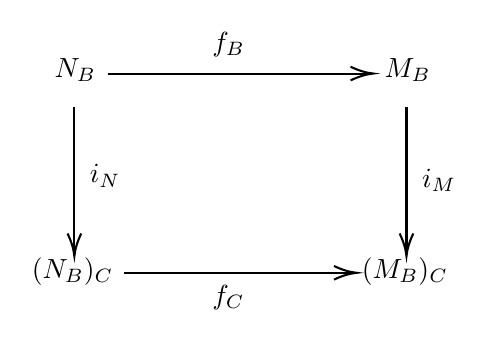
\begin{tikzpicture}[x=0.75pt,y=0.75pt,yscale=-1,xscale=1]
%uncomment if require: \path (0,476); %set diagram left start at 0, and has height of 476

%Straight Lines [id:da4966514445313652] 
\draw    (216,160) -- (342,160) ;
\draw [shift={(344,160)}, rotate = 180] [color={rgb, 255:red, 0; green, 0; blue, 0 }  ][line width=0.75]    (10.93,-3.29) .. controls (6.95,-1.4) and (3.31,-0.3) .. (0,0) .. controls (3.31,0.3) and (6.95,1.4) .. (10.93,3.29)   ;
%Straight Lines [id:da9996774197216416] 
\draw    (200,176) -- (200,246) ;
\draw [shift={(200,248)}, rotate = 270] [color={rgb, 255:red, 0; green, 0; blue, 0 }  ][line width=0.75]    (10.93,-3.29) .. controls (6.95,-1.4) and (3.31,-0.3) .. (0,0) .. controls (3.31,0.3) and (6.95,1.4) .. (10.93,3.29)   ;
%Straight Lines [id:da49733541515705393] 
\draw    (360,176) -- (360,246) ;
\draw [shift={(360,248)}, rotate = 270] [color={rgb, 255:red, 0; green, 0; blue, 0 }  ][line width=0.75]    (10.93,-3.29) .. controls (6.95,-1.4) and (3.31,-0.3) .. (0,0) .. controls (3.31,0.3) and (6.95,1.4) .. (10.93,3.29)   ;
%Straight Lines [id:da8610440093860443] 
\draw    (224,256) -- (334,256) ;
\draw [shift={(336,256)}, rotate = 180] [color={rgb, 255:red, 0; green, 0; blue, 0 }  ][line width=0.75]    (10.93,-3.29) .. controls (6.95,-1.4) and (3.31,-0.3) .. (0,0) .. controls (3.31,0.3) and (6.95,1.4) .. (10.93,3.29)   ;

% Text Node
\draw (189,151.4) node [anchor=north west][inner sep=0.75pt]    {$N_{B}$};
% Text Node
\draw (348,151.4) node [anchor=north west][inner sep=0.75pt]    {$M_{B}$};
% Text Node
\draw (178,247.4) node [anchor=north west][inner sep=0.75pt]    {$( N_{B})_{C}$};
% Text Node
\draw (337,247.4) node [anchor=north west][inner sep=0.75pt]    {$( M_{B})_{C}$};
% Text Node
\draw (265,138.4) node [anchor=north west][inner sep=0.75pt]    {$f_{B}$};
% Text Node
\draw (206,202.4) node [anchor=north west][inner sep=0.75pt]    {$i_{N}$};
% Text Node
\draw (366,204.4) node [anchor=north west][inner sep=0.75pt]    {$i_{M}$};
% Text Node
\draw (265,260.4) node [anchor=north west][inner sep=0.75pt]    {$f_{C}$};


\end{tikzpicture}
\end{center}
where the map $f_C$ is also injective since $g\circ f$ is flat. Therefore $f_B$ must be injective and hence $f$ is flat.
\end{proof}
\begin{problem}\em
Let $f:A\to B$ be a flat homomorphism of rings, let $\mathfrak{q}$ be a prime ideal of $B$ and let $\mathfrak{p}=\mathfrak{q}^c$. Then $f^*:\mathrm{Spec}(B_\mathfrak{q})\to\mathrm{Spec}(A_\mathfrak{p})$ is surjective.
\end{problem}
\begin{proof}
It suffices to show that $B_\mathfrak{q}$ is faithfully flat over $A_\mathfrak{p}$. First note that $B$ is a flat module over $A$, hence $B_\mathfrak{p}$ is a flat module over $A_\mathfrak{p}$. Since $\mathfrak{q}=\mathfrak{p}^c$, we have $\mathfrak{q}^e=\mathfrak{p}^{ce}\subset\mathfrak{p}$, hence $B_\mathfrak{q}$ is a localization of $A_\mathfrak{p}$ module $B_\mathfrak{p}$, and hence a flat $A_\mathfrak{p}$ module. Now we show the faithfulness. Suppose $\mathfrak{m}$ is a maximal ideal of $A_\mathfrak{p}$. Let $\overline{f}$ be the following composition: 
$$
A_{\mathfrak{p}}\longrightarrow B_{\mathfrak{p}}\longrightarrow B_{\mathfrak{q}},
$$
suppose $a/s\in\mathfrak{m}$, then $\overline{f}(a/s)=f(p)/f(s)\in f(\mathfrak{p})^{-1}B_\mathfrak{q}$, which implies $\mathfrak{m}^e\ne (1)$ and the proof is finished.
\end{proof}
\begin{problem}\em
Let $A$ be a ring, $M$ an $A$-module. The \textbf{support} of $M$ is defined to be the set $\mathrm{Supp}(M)$ of prime ideals $\mathfrak{p}$ of $A$ such that $M_\mathfrak{p}\ne 0$. Prove the following results:\par
(i) $M\ne 0$ if and only if $\mathrm{Supp}(M)\ne\emptyset$.\par
(ii) $V(\mathfrak{a})=\mathrm{Supp}(A/\mathfrak{a})$.\par
(iii) If $0\longrightarrow M^{\prime}\longrightarrow M\longrightarrow M^{\prime\prime}\longrightarrow 0$ is a short exact sequence, then $\mathrm{Supp}(M)=\mathrm{Supp}(M^\prime)\cup\mathrm{Supp}(M^{\prime\prime})$.\par
(iv) If $M=\sum M_i$, then $\mathrm{Supp}(M)=\bigcup\mathrm{Supp}(M_i)$.\par
(v) If $M$ is finitely generated, then $\mathrm{Supp}(M)=V(\mathrm{Ann}(M))$.\par
(vi) If $M$ and $N$ are finitely generated, then $\mathrm{Supp}(M\otimes_AN)=\mathrm{Supp}(M)\cap\mathrm{Supp}(N)$.\par
(vii) If $M$ is finitely generated and $\mathfrak{a}$ a prime ideal of $A$, then $\mathrm{Supp}(M/\mathfrak{a}M)=V(\mathfrak{a}+\mathrm{Ann}(M))$.\par
(viii) If $f:A\to B$ is a ring homomorphism and $M$ is a finitely generated $A$-module, then $\mathrm{Supp}(B\otimes_AM)=f^{*-1}(\mathrm{Supp}(M))$.
\end{problem}
\begin{proof}
(i) Suppose $M=0$. Then for all $\mathfrak{p}$ we have $M_\mathfrak{p}=0$. Note that these two statements are equivalent.\par
(ii) Let $\mathfrak{p}$ be a prime ideal. Define $S=A-\mathfrak{p}$. Then 
$$
\begin{aligned}
\mathfrak{p}\in V(\mathfrak{a}) & \iff \mathfrak{a}\cap S=0 \\
& \iff \text{There is no such }t,s\in S\text{ such that }ts=ta\in\mathfrak{a}\cap S \\
& \iff 1/1\ne a/s\in S^{-1}\mathfrak{a}\text{ for all }a/s\in S^{-1}\mathfrak{a} \\
& \iff S^{-1}\mathfrak{a}\text{ has no identity} \\
& \iff S^{-1}\mathfrak{a}\ne S^{-1}A \\
& \iff S^{-1}A/S^{-1}\mathfrak{a}=(A/\mathfrak{a})_\mathfrak{p}\ne 0 \\
& \iff \mathfrak{p}\in\mathrm{Supp}(A/\mathfrak{a}).
\end{aligned}
$$\par
(iii) Suppose $\mathfrak{p}\in\mathrm{Supp}(M)$. Then $M_\mathfrak{p}\ne 0$ and hence the exact sequence 
$$
0\longrightarrow M_{\mathfrak{p}}^{\prime}\longrightarrow M_{\mathfrak{p}}\longrightarrow M_{\mathfrak{p}}^{\prime\prime}\longrightarrow 0
$$
is also an exact sequence with $M_\mathfrak{p}\ne 0$. Therefore $M_\mathfrak{p}^\prime$ and $M_\mathfrak{p}^{\prime\prime}$ are both nonzero and hence $\mathfrak{p}\in\mathrm{Supp}(M^\prime)\cup\mathrm{Supp}(M^{\prime\prime})$. The converse follows analogously.\par
(iv) We first show that $S^{-1}-$ is commutative with the direct sum. It suffices to note that 
$$
S^{-1}\left( \bigoplus_{i=1}^n{M_i} \right) \cong S^{-1}A\otimes _A\left( \bigoplus_{i=1}^n{M_i} \right) \cong \bigoplus_{i=1}^n{\left( S^{-1}A\otimes _AM_i \right)}\cong \bigoplus_{i=1}^n{S^{-1}M_i}.
$$
Now we have  
$$
\begin{aligned}
\mathfrak{p} & \iff M_\mathfrak{p}\ne 0 \\
& \iff \left(\sum M_i\right)_\mathfrak{p}\ne 0 \\
& \iff (M_i)_\mathfrak{p}\ne 0\text{ for some index }i \\
& \iff \mathfrak{p}\in\bigcup\mathrm{Supp}(M_i).
\end{aligned}
$$\par
(v) Suppose $M\cong\bigoplus_{i=1}^nAx_i\cong\bigoplus_{i=1}^nA/\mathfrak{a}_i$. Then 
$$
\mathrm{Supp}\left( M \right) =\mathrm{Supp}\left( \bigoplus_{i=1}^n{A/\mathfrak{a} _i} \right) =\bigcup_{i=1}^n{\mathrm{Supp}\left( A/\mathfrak{a} _i \right)}=\bigcup_{i=1}^n{V\left( \mathfrak{a} _i \right)}=V\left( \bigcap_{i=1}^n{\mathfrak{a} _i} \right) .
$$
Now if $a\in\mathrm{Ann}(M)$, then the map $A\to Ax_i$ gives $a\mapsto 0$. Therefore $a\in\bigcap_{i=1}^n\mathfrak{a}_i$. Conversely, suppose $a\in\bigcap_{i=1}^n\mathfrak{a}_i$, then $ax_i=0$ for every generator $x_i$, hence $a\in\mathrm{Ann}(M)$. Therefore $\bigcap_{i=1}^n\mathfrak{a}_i=\mathrm{Ann}(M)$ and hence $\mathrm{Supp}(M)=V(\mathrm{Ann}(M))$.\par
(vi) Suppose $\mathfrak{p}\in\mathrm{Supp}(M\otimes_AN)$, then we have $(M\otimes_AN)_\mathfrak{p}\ne 0$. Note that 
$\left( M\otimes _AN \right) _{\mathfrak{p}}=M_{\mathfrak{p}}\otimes _AN_{\mathfrak{p}}$ and both $N$ and $M$ are finitely generated, we have both $M_\mathfrak{p}$ and $N_\mathfrak{p}\ne 0$, whence $\mathfrak{p}\in\mathrm{Supp}(M)\cap\mathrm{Supp}(N)$. The converse follows analogously.\par
(vii) Note that 
$$
\begin{aligned}
\mathrm{Supp}\left( M/\mathfrak{a} M \right) &=\mathrm{Supp}\left( A/\mathfrak{a} \otimes _AM \right) =\mathrm{Supp}\left( A/\mathfrak{a} \right) \cap \mathrm{Supp}\left( M \right) 
\\
&=V\left( \mathfrak{a} \right) \cap V\left( \mathrm{Ann}\left( M \right) \right) =V\left( \mathfrak{a} \cup \mathrm{Ann}\left( M \right) \right) =V\left( \mathfrak{a} +\mathrm{Ann}\left( M \right) \right) ,
\end{aligned}
$$
which finished the proof.\par
(viii) Suppose $\mathfrak{q}\in\mathrm{Spec}(B)$ and $\mathfrak{p}=\mathfrak{q}^c$. It suffices to show that $\mathfrak{q}\in\mathrm{Supp}(B\otimes_AM)$ if and only if $\mathfrak{p}\in\mathrm{Supp}(M)$. Suppose $\mathfrak{q}\in\mathrm{Supp}(B\otimes_AM)$. Then since 
$$
\left( B\otimes _AM \right) _{\mathfrak{q}}\cong B_{\mathfrak{q}}\otimes _BB\otimes _AM\cong B_{\mathfrak{q}}\otimes _AM\cong B_{\mathfrak{q}}\otimes _{A_{\mathfrak{p}}}A_{\mathfrak{p}}\otimes _AM\cong B_{\mathfrak{q}}\otimes _{A_{\mathfrak{p}}}M_{\mathfrak{p}},
$$
we have $B_{\mathfrak{q}}\otimes _{A_{\mathfrak{p}}}M_{\mathfrak{p}}\ne 0$, hence $\mathfrak{p}\in\mathrm{Supp}(M)$. Conversely, suppose $(B\otimes_AM)_\mathfrak{q}=0$, it suffices to show that $M_\mathfrak{p}=0$. Since 
$$
0=\left( B\otimes _AM \right) _{\mathfrak{q}}=B_{\mathfrak{q}}\otimes _{A_{\mathfrak{p}}}M_{\mathfrak{p}},
$$
suppose $x_1,\cdots,x_n$ be a set of generators of $M$, then we have $(1/1)\otimes(x_i/1)=0$. Therefore there exists some $N_i\subset B$ such that $1/1\in N_i$, $(1/1)\otimes(x_i/1)=0$ in $N_i\otimes_AM$. Define $N=\bigoplus_{i=1}^nN_i$, then $(N\otimes_AM)_\mathfrak{q}=0$. Since both $N$ and $M$ are finitely generated and $1/1\in N$, we must have $M_\mathfrak{q}=0$, which finished the proof. 
\end{proof}
\begin{problem}\em
Let $f:A\to B$ be a ring homomorphism, $f^*:\mathrm{Spec}(B)\to\mathrm{Spec}(A)$ the associated mapping. Show that \par
(i) Every prime ideal of $A$ is a contracted ideal if and only if $f^*$ is surjective.\par
(ii) Every prime ideal of $B$ is an extended ideal implies $f^*$ is injective. Is the converse true?
\end{problem}
\begin{proof}
(i) Suppose every prime ideal of $A$ is a contracted ideal of $B$. Then for all $\mathfrak{p}\in\mathrm{Spec}(A)$, there exists some $\mathfrak{q}\in\mathrm{Spec}(B)$ such that $f^*(\mathfrak{q})=\mathfrak{p}$, whence $f^*$ is surjective. Conversely, suppose $f^*$ is surjective, then for all $\mathfrak{p}\in\mathrm{Spec}(A)$, there exists some $\mathfrak{q}\in\mathrm{Spec}(B)$ such that $f^*(\mathfrak{q})=\mathfrak{p}$, i.e. $\mathfrak{q}^c=\mathfrak{p}$.\par
(ii) Suppose every prime ideal of $B$ is an extended ideal of $B$. Then let $\mathfrak{p}\in\mathrm{Ker}f^*$, there exists some $\mathfrak{q}\in\mathrm{Spec}(B)$ such that $\mathfrak{q}=\mathfrak{p}^e$. Therefore $f^*(\mathfrak{q})=\mathfrak{q}^c=\mathfrak{p}^{ec}\supset\mathfrak{p}$. However $0=f^*(\mathfrak{q})$, whence $\mathfrak{p}=0$ and hence $\mathfrak{q}=0^e=0$.\par
However, the converse is false. For a counterexample, consider the ring $B=A[x]/(x^2)$, where $A$ is another ring. We claim that every prime ideal $\mathfrak{p}$ in $A$ has its extension $\mathfrak{p}^e$ not a prime, and hence every prime $\mathfrak{q}$ of $A[x]/(x^2)$ is not an extension of some prime ideals $\mathfrak{p}$ of $A$. Suppose $\mathfrak{p}\in\mathrm{Spec}(A)$. Then 
$$
\mathfrak{p} ^e=\left< \mathfrak{p} \right> =\mathfrak{p} A\left[ x \right] /\left( x^2 \right) =\left\{ a+bx:a,b\in \mathfrak{p} \right\} ,
$$
which is not a prime ideal. However, on the other hand, we show that there is a one-to-one correspondence between prime ideals of $A$ and $B$. Indeed, suppose $\mathfrak{p}$ is a prime ideal of $A$. Then its inverse is a prime ideal contained in $(x^2)$. Conversely, suppose $\mathfrak{q}$ is a prime ideal of $B$, then it contains $0=x^2$, thus $x$ is in the prime ideal. Therefore every prime ideal in $B$ is some contraction of $A$. Hence if we consider the map $\phi:A\to B$, we have $\phi^*$ is injective (actually an isomorphism), however no prime ideal of $B$ is an extended ideal of $A$.
\end{proof}
\begin{problem}\em
(i) Let $A$ be a ring, $S$ a multiplicative subset of $A$, and $\phi:A\to S^{-1}A$ the canonical homomorphism. Show that $\phi^*:\mathrm{Spec}(S^{-1}A)\to\mathrm{Spec}(A)$ is a homeomorphism of $\mathrm{Spec}(S^{-1}A)$ onto its image in $X=\mathrm{Spec}(A)$. Let this image denoted by $S^{-1}X$. In particular, if $f\in A$, the image of $\mathrm{Spec}(A_f)$ in $X$ is the basic open set $X_f$.\par
(ii) Let $f:A\to B$ be a ring homomorphism. Let $X=\mathrm{Spec}(A)$ and $Y=\mathrm{Spec}(B)$, and let $f^*:Y\to X$ be the mapping associated with $f$. Identifying $\mathrm{Spec}(S^{-1}A)$ with its canonical image $S^{-1}X$ in $X$, and $\mathrm{Spec}(S^{-1}B)$ with its canonical image $S^{-1}Y$ in $Y$. Show that $S^{-1}f^*:\mathrm{Spec}(S^{-1}B)\to\mathrm{Spec}(S^{-1}A)$ is the restriction of $f^*$ to $S^{-1}Y$, and that $S^{-1}Y=f^{*-1}(S^{-1}X)$.\par
(iii) Let $\mathfrak{a}$ be an ideal of $A$ and let $\mathfrak{b}=\mathfrak{a}^e$ be its extension in $B$. Let $\overline{f}:A/\mathfrak{a}\to B/\mathfrak{b}$ be the homomorphism induced by $f$. If $\mathrm{Spec}(A/\mathfrak{a})$ is identified with its canonical image $V(\mathfrak{a})$ in $X$, and $\mathrm{Spec}(B/\mathfrak{b})$ with its image $V(\mathfrak{b})$ in $Y$, show that $\overline{f}^*$ is the restriction of $f^*$ to $V(\mathfrak{b})$.\par
(iv) Let $\mathfrak{p}$ be a prime ideal of $A$. Take $S=A-\mathfrak{p}$ in (ii) and then reduce mod $S^{-1}\mathfrak{p}$ as in (iii). Deduce that the subspace $f^{*-1}(\mathfrak{p})$ of $Y$ naturally homeomorphic to $\mathrm{Spec}(B_\mathfrak{p}/\mathfrak{p}B_\mathfrak{p})=\mathrm{Spec}(\kappa(\mathfrak{p})\otimes_AB)$, where $\kappa(\mathfrak{p})$ is the residue field of the local ring $A_\mathfrak{p}$.\par
$\mathrm{Spec}(\kappa(\mathfrak{p})\otimes_AB)$ is called the \textbf{fiber} of $f^*$ over $\mathfrak{p}$.
\end{problem}
\begin{proof}
(i) We first mention a result: If $\mathfrak{p}$ is a prime ideal such that $\mathfrak{p}\cap S=\emptyset$, then $\mathfrak{p}^{ec}=\mathfrak{p}$. To see this, since there is a one-to-one correspondence between the prime ideals of $A$ that does not meet $S$ and the ideals of $S^{-1}A$, we may suppose $\mathfrak{p}=\mathfrak{q}^c$ for some $\mathfrak{q}\in\mathrm{Spec}(S^{-1}A)$. Therefore $\mathfrak{p}^{ec}=\mathfrak{q}^{cec}=\mathfrak{q}^c=\mathfrak{p}$, which finished the proof. We now show that $\phi^*$ is a homeomorphism. We have shown in Exercise 7.7 that $\phi^*$ is continuous. It is also clear that the prime ideals of $A$ that does not meet $S$ is one-to-one correspondent with the ideals of $S^{-1}A$. Now it remains to show that the inverse of $\phi^*$ is continuous. We show the image of every closed subset of $\mathrm{Spec}(S^{-1}A)$ is also closed in $\mathrm{Spec}(A)$. Suppose $V(\mathfrak{a}^e)$ is a closed subset in $\mathrm{Spec}(S^{-1}A)$, we are going to proof that $\phi^*:V(\mathfrak{a}^e)\mapsto V(\mathfrak{a})\cap S^{-1}X$. To do this, suppose first $\mathfrak{a}^e\subset\mathfrak{p}^e$, then $\mathfrak{a}\subset\mathfrak{a}^{ec}\subset\mathfrak{p}^{ec}=\mathfrak{p}$, where the last equality follows from the preceding fact. Conversely, suppose $\mathfrak{a}\subset\mathfrak{p}$ for some $\mathfrak{p}\cap S=\emptyset$. Then $\mathfrak{a}^e\subset\mathfrak{p}^e\ne (1)$, which finished the proof.\par
(ii) It suffices to show that the following diagram is commute: 
\begin{center}


\tikzset{every picture/.style={line width=0.75pt}} %set default line width to 0.75pt        

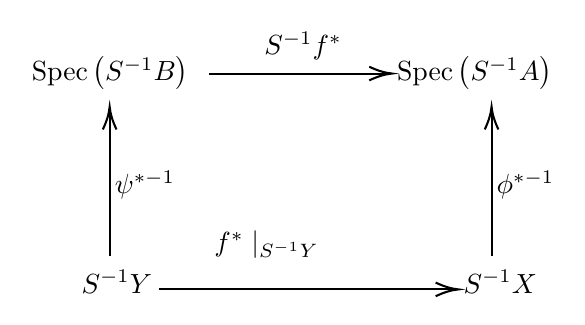
\begin{tikzpicture}[x=0.75pt,y=0.75pt,yscale=-1,xscale=1]
%uncomment if require: \path (0,476); %set diagram left start at 0, and has height of 476

%Straight Lines [id:da4088698840446132] 
\draw    (256,144) -- (342,144) ;
\draw [shift={(344,144)}, rotate = 180] [color={rgb, 255:red, 0; green, 0; blue, 0 }  ][line width=0.75]    (10.93,-3.29) .. controls (6.95,-1.4) and (3.31,-0.3) .. (0,0) .. controls (3.31,0.3) and (6.95,1.4) .. (10.93,3.29)   ;
%Straight Lines [id:da07164472267101019] 
\draw    (392,232) -- (392,162) ;
\draw [shift={(392,160)}, rotate = 90] [color={rgb, 255:red, 0; green, 0; blue, 0 }  ][line width=0.75]    (10.93,-3.29) .. controls (6.95,-1.4) and (3.31,-0.3) .. (0,0) .. controls (3.31,0.3) and (6.95,1.4) .. (10.93,3.29)   ;
%Straight Lines [id:da4491814482984402] 
\draw    (208,232) -- (208,162) ;
\draw [shift={(208,160)}, rotate = 90] [color={rgb, 255:red, 0; green, 0; blue, 0 }  ][line width=0.75]    (10.93,-3.29) .. controls (6.95,-1.4) and (3.31,-0.3) .. (0,0) .. controls (3.31,0.3) and (6.95,1.4) .. (10.93,3.29)   ;
%Straight Lines [id:da8080773307890523] 
\draw    (232,248) -- (374,248) ;
\draw [shift={(376,248)}, rotate = 180] [color={rgb, 255:red, 0; green, 0; blue, 0 }  ][line width=0.75]    (10.93,-3.29) .. controls (6.95,-1.4) and (3.31,-0.3) .. (0,0) .. controls (3.31,0.3) and (6.95,1.4) .. (10.93,3.29)   ;

% Text Node
\draw (169,134.4) node [anchor=north west][inner sep=0.75pt]    {$\mathrm{Spec}\left( S^{-1} B\right)$};
% Text Node
\draw (345,134.4) node [anchor=north west][inner sep=0.75pt]    {$\mathrm{Spec}\left( S^{-1} A\right)$};
% Text Node
\draw (377,237.4) node [anchor=north west][inner sep=0.75pt]    {$S^{-1} X$};
% Text Node
\draw (193,237.4) node [anchor=north west][inner sep=0.75pt]    {$S^{-1} Y$};
% Text Node
\draw (281,122.4) node [anchor=north west][inner sep=0.75pt]    {$S^{-1} f^{*}$};
% Text Node
\draw (257,218.4) node [anchor=north west][inner sep=0.75pt]    {$f^{*} \mid _{S^{-1}Y}$};
% Text Node
\draw (393,189.4) node [anchor=north west][inner sep=0.75pt]    {$\phi ^{*-1}$};
% Text Node
\draw (209,189.4) node [anchor=north west][inner sep=0.75pt]    {$\psi ^{*-1}$};


\end{tikzpicture}
\end{center}
Suppose $\mathfrak{q}\in S^{-1}Y$, then we have $f^*(\mathfrak{q})=f^{-1}(\mathfrak{q})$, which is an ideal in $S^{-1}X$. Therefore 
$$
\phi ^{*-1}\circ f^*\mid _{S^{-1}Y}\left( \mathfrak{q} \right) =\phi ^{*-1}\left( f^{-1}\left( \mathfrak{q} \right) \right) =\left( \left\{ a/1:f\left( a \right) \in \mathfrak{q} \right\} \right) .
$$
Now for another route, we have $\psi^{*-1}(\mathfrak{q})$ is the ideal generated by $\{a/1:a\in\mathfrak{q}\}$, whence 
$$
S^{-1}f^*\circ \psi ^{*-1}\left( \mathfrak{q} \right) =\left( \left\{ a/1:f\left( a \right) \in \mathfrak{q} \right\} \right) ,
$$
hence we have the diagram commutative and the proof is finished.\par
(iii) It suffices to show that the following diagram is commutative: 
\begin{center}


\tikzset{every picture/.style={line width=0.75pt}} %set default line width to 0.75pt        

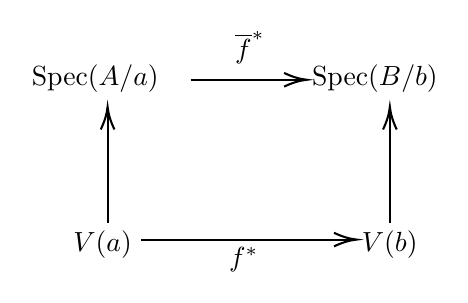
\begin{tikzpicture}[x=0.75pt,y=0.75pt,yscale=-1,xscale=1]
%uncomment if require: \path (0,476); %set diagram left start at 0, and has height of 476

%Straight Lines [id:da9694501417798485] 
\draw    (224,216) -- (326,216) ;
\draw [shift={(328,216)}, rotate = 180] [color={rgb, 255:red, 0; green, 0; blue, 0 }  ][line width=0.75]    (10.93,-3.29) .. controls (6.95,-1.4) and (3.31,-0.3) .. (0,0) .. controls (3.31,0.3) and (6.95,1.4) .. (10.93,3.29)   ;
%Straight Lines [id:da1752610206989369] 
\draw    (208,208) -- (208,154) ;
\draw [shift={(208,152)}, rotate = 90] [color={rgb, 255:red, 0; green, 0; blue, 0 }  ][line width=0.75]    (10.93,-3.29) .. controls (6.95,-1.4) and (3.31,-0.3) .. (0,0) .. controls (3.31,0.3) and (6.95,1.4) .. (10.93,3.29)   ;
%Straight Lines [id:da08695868041479371] 
\draw    (344,208) -- (344,154) ;
\draw [shift={(344,152)}, rotate = 90] [color={rgb, 255:red, 0; green, 0; blue, 0 }  ][line width=0.75]    (10.93,-3.29) .. controls (6.95,-1.4) and (3.31,-0.3) .. (0,0) .. controls (3.31,0.3) and (6.95,1.4) .. (10.93,3.29)   ;
%Straight Lines [id:da4442804456162608] 
\draw    (248,139) -- (302,139) ;
\draw [shift={(304,139)}, rotate = 180] [color={rgb, 255:red, 0; green, 0; blue, 0 }  ][line width=0.75]    (10.93,-3.29) .. controls (6.95,-1.4) and (3.31,-0.3) .. (0,0) .. controls (3.31,0.3) and (6.95,1.4) .. (10.93,3.29)   ;

% Text Node
\draw (190,210.4) node [anchor=north west][inner sep=0.75pt]    {$V(\mathfrak{a})$};
% Text Node
\draw (329,210.4) node [anchor=north west][inner sep=0.75pt]    {$V(\mathfrak{b})$};
% Text Node
\draw (170,130.4) node [anchor=north west][inner sep=0.75pt]    {$\mathrm{Spec}( A/\mathfrak{a})$};
% Text Node
\draw (305,130.4) node [anchor=north west][inner sep=0.75pt]    {$\mathrm{Spec}( B/\mathfrak{b})$};
% Text Node
\draw (265,218.4) node [anchor=north west][inner sep=0.75pt]    {$f^{*}$};
% Text Node
\draw (268,114.4) node [anchor=north west][inner sep=0.75pt]    {$\overline{f}^{*}$};


\end{tikzpicture}
\end{center}
The proof of which is similar to (ii) and we skip the details.\par
(iv) Note that 
$$
S^{-1}A/S^{-1}\mathfrak{p} \cong S^{-1}\left( A/\mathfrak{p} \right) =\left( A/\mathfrak{p} \right) _{\mathfrak{p}}=A_{\mathfrak{p}}/\mathfrak{p} A_{\mathfrak{p}},
$$
which is the same for $B$, we have the following diagram: 
\begin{center}


\tikzset{every picture/.style={line width=0.75pt}} %set default line width to 0.75pt        

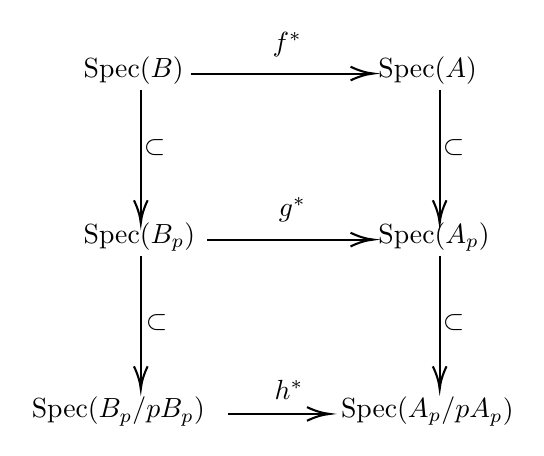
\begin{tikzpicture}[x=0.75pt,y=0.75pt,yscale=-1,xscale=1]
%uncomment if require: \path (0,476); %set diagram left start at 0, and has height of 476

%Straight Lines [id:da7331249318884367] 
\draw    (208,128) -- (208,190) ;
\draw [shift={(208,192)}, rotate = 270] [color={rgb, 255:red, 0; green, 0; blue, 0 }  ][line width=0.75]    (10.93,-3.29) .. controls (6.95,-1.4) and (3.31,-0.3) .. (0,0) .. controls (3.31,0.3) and (6.95,1.4) .. (10.93,3.29)   ;
%Straight Lines [id:da5180820866302538] 
\draw    (352,128) -- (352,190) ;
\draw [shift={(352,192)}, rotate = 270] [color={rgb, 255:red, 0; green, 0; blue, 0 }  ][line width=0.75]    (10.93,-3.29) .. controls (6.95,-1.4) and (3.31,-0.3) .. (0,0) .. controls (3.31,0.3) and (6.95,1.4) .. (10.93,3.29)   ;
%Straight Lines [id:da07133466719075199] 
\draw    (208,208) -- (208,270) ;
\draw [shift={(208,272)}, rotate = 270] [color={rgb, 255:red, 0; green, 0; blue, 0 }  ][line width=0.75]    (10.93,-3.29) .. controls (6.95,-1.4) and (3.31,-0.3) .. (0,0) .. controls (3.31,0.3) and (6.95,1.4) .. (10.93,3.29)   ;
%Straight Lines [id:da4322175332278939] 
\draw    (352,208) -- (352,270) ;
\draw [shift={(352,272)}, rotate = 270] [color={rgb, 255:red, 0; green, 0; blue, 0 }  ][line width=0.75]    (10.93,-3.29) .. controls (6.95,-1.4) and (3.31,-0.3) .. (0,0) .. controls (3.31,0.3) and (6.95,1.4) .. (10.93,3.29)   ;
%Straight Lines [id:da2533120990555766] 
\draw    (232,120) -- (318,120) ;
\draw [shift={(320,120)}, rotate = 180] [color={rgb, 255:red, 0; green, 0; blue, 0 }  ][line width=0.75]    (10.93,-3.29) .. controls (6.95,-1.4) and (3.31,-0.3) .. (0,0) .. controls (3.31,0.3) and (6.95,1.4) .. (10.93,3.29)   ;
%Straight Lines [id:da20741230504364472] 
\draw    (240,200) -- (318,200) ;
\draw [shift={(320,200)}, rotate = 180] [color={rgb, 255:red, 0; green, 0; blue, 0 }  ][line width=0.75]    (10.93,-3.29) .. controls (6.95,-1.4) and (3.31,-0.3) .. (0,0) .. controls (3.31,0.3) and (6.95,1.4) .. (10.93,3.29)   ;
%Straight Lines [id:da10419584755332689] 
\draw    (250,284) -- (297,284) ;
\draw [shift={(299,284)}, rotate = 180] [color={rgb, 255:red, 0; green, 0; blue, 0 }  ][line width=0.75]    (10.93,-3.29) .. controls (6.95,-1.4) and (3.31,-0.3) .. (0,0) .. controls (3.31,0.3) and (6.95,1.4) .. (10.93,3.29)   ;

% Text Node
\draw (179,110.4) node [anchor=north west][inner sep=0.75pt]    {$\mathrm{Spec}( B)$};
% Text Node
\draw (321,110.4) node [anchor=north west][inner sep=0.75pt]    {$\mathrm{Spec}( A)$};
% Text Node
\draw (179,190.4) node [anchor=north west][inner sep=0.75pt]    {$\mathrm{Spec}( B_{\mathfrak{p}})$};
% Text Node
\draw (321,190.4) node [anchor=north west][inner sep=0.75pt]    {$\mathrm{Spec}( A_{\mathfrak{p}})$};
% Text Node
\draw (154,274.4) node [anchor=north west][inner sep=0.75pt]    {$\mathrm{Spec}( B_{\mathfrak{p}} /\mathfrak{p} B_{\mathfrak{p}})$};
% Text Node
\draw (303.03,274.25) node [anchor=north west][inner sep=0.75pt]  [rotate=-0.17]  {$\mathrm{Spec}( A_{\mathfrak{p}} /\mathfrak{p} A_{\mathfrak{p}})$};
% Text Node
\draw (208,150.4) node [anchor=north west][inner sep=0.75pt]    {$\subset $};
% Text Node
\draw (209,234.4) node [anchor=north west][inner sep=0.75pt]    {$\subset $};
% Text Node
\draw (352,150.4) node [anchor=north west][inner sep=0.75pt]    {$\subset $};
% Text Node
\draw (352,234.4) node [anchor=north west][inner sep=0.75pt]    {$\subset $};
% Text Node
\draw (270,98.4) node [anchor=north west][inner sep=0.75pt]    {$f^{*}$};
% Text Node
\draw (273,178.4) node [anchor=north west][inner sep=0.75pt]    {$g^{*}$};
% Text Node
\draw (271,266.4) node [anchor=north west][inner sep=0.75pt]    {$h^{*}$};


\end{tikzpicture}
\end{center}
where $g^*$ and $h^*$ are the restrictions of $f^*$ by the preceding discussion. By the commutative diagram above we have $\mathrm{Spec}(A_\mathfrak{p}/\mathfrak{p}A_\mathfrak{p})$ corresponds to the prime ideal in $\mathrm{Spec}(A_\mathfrak{p})$ that contain $\mathfrak{p}A_\mathfrak{p}$, and again corresponds to the prime ideal in $\mathrm{Spec}(A)$ that contains $\mathfrak{p}$, hence $\mathrm{Spec}(A_\mathfrak{p}/\mathfrak{p}A_\mathfrak{p})$ corresponds to the primes in $\mathrm{Spec}(A)$ that contained $\mathfrak{p}$ and contains in $\mathfrak{p}$, which is the singleton $\{\mathfrak{p}\}$. Thus the space $\mathrm{Spec}(B_\mathfrak{p}/\mathfrak{p}B_\mathfrak{p})$ is identified with the preimage $f^{*-1}(\mathfrak{p})$ . Now note that 
$$
\begin{aligned}
\mathrm{Spec}\left( \kappa \left( \mathfrak{p} \right) \otimes _AB \right) &=\mathrm{Spec}\left( A_{\mathfrak{p}}/\mathfrak{p} A_{\mathfrak{p}}\otimes _AB \right) \cong \mathrm{Spec}\left( S^{-1}\left( A/\mathfrak{p} \right) \otimes _AB \right) 
\\
&\cong \mathrm{Spec}\left( S^{-1}\left( A/\mathfrak{p} \right) \otimes _{A/\mathfrak{p}}A/\mathfrak{p} \otimes _AB \right) \cong \mathrm{Spec}\left( S^{-1}\left( A/\mathfrak{p} \right) \otimes _{A/\mathfrak{p}}B/\mathfrak{p} B \right) 
\\
&\cong \mathrm{Spec}\left( S^{-1}\left( B/\mathfrak{p} B \right) \right) \cong \mathrm{Spec}\left( B_{\mathfrak{p}}/\mathfrak{p} B_{\mathfrak{p}} \right) ,
\end{aligned}
$$
which finished the proof.
\end{proof}
\begin{problem}\em
Let $A$ be a ring and $\mathfrak{p}$ a prime ideal of $A$. Then the canonical image of $\mathrm{Spec}(A_\mathfrak{p})$ in $\mathrm{Spec}(A)$ is equal to the intersection of all the open neighborhoods of $\mathfrak{p}$ in $\mathrm{Spec}(A)$.
\end{problem}
\begin{proof}
Note that 
$$
\begin{aligned}
\mathfrak{q}\in\mathrm{Spec}(A_\mathfrak{p}) & \iff \mathfrak{q}\in\mathrm{Spec}(A)\text{ and }\mathfrak{q}\supset\mathfrak{p} \\
& \iff \mathfrak{q}\in X_f\text{ for all }f\text{ such that }\mathfrak{p}\in X_f \\
& \iff \mathfrak{q}\in\bigcap_{\mathfrak{p}\in X_f}X_f,
\end{aligned}
$$
which implies $\mathfrak{q}\in\bigcap_{\mathfrak{p}\in X_f}X_f$.
\end{proof}
\begin{note}\em
Note that this exercise gives an illustration of the geometric interpretation of localization.
\end{note}
\begin{problem}\em
Let $A$ be a ring, let $X=\mathrm{Spec}(A)$ and let $U$ be a basic open set in $X$ (i.e. $U=X_f$ for some $f\in A$).\par
(i) If $U=X_f$, show that the ring $A(U)=A_f$ depends only on $U$ and not on $f$.\par
(ii) Let $U^\prime=X_g$ be another basic open set such that $U^\prime\subset U$. Show that there is an equation of the form $g^n=uf$ for some integer $n>0$ and some $u\in A$, and use this to define a homomorphism $\rho:A(U)\to A(U^\prime)$ by mapping $a/f^m$ to $au^m/ag^m$. Show that $\rho$ depends only on $U$ and $U^\prime$. This homomorphism is called the \textbf{restriction homomorphism}.\par
(iii) If $U=U^\prime$, then $\rho$ is the identity map.\par
(iv) If $U\supset U^\prime\supset U^{\prime\prime}$ are basic open sets in $X$, show that the diagram 
\begin{center}


\tikzset{every picture/.style={line width=0.75pt}} %set default line width to 0.75pt        

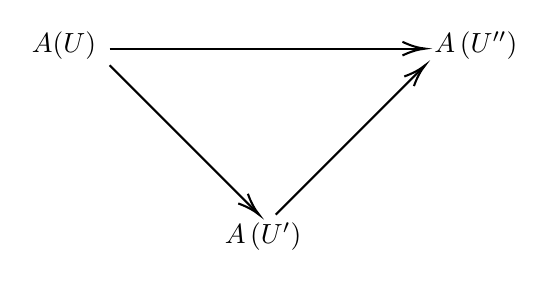
\begin{tikzpicture}[x=0.75pt,y=0.75pt,yscale=-1,xscale=1]
%uncomment if require: \path (0,476); %set diagram left start at 0, and has height of 476

%Straight Lines [id:da5484788379249899] 
\draw    (176,144) -- (326,144) ;
\draw [shift={(328,144)}, rotate = 180] [color={rgb, 255:red, 0; green, 0; blue, 0 }  ][line width=0.75]    (10.93,-3.29) .. controls (6.95,-1.4) and (3.31,-0.3) .. (0,0) .. controls (3.31,0.3) and (6.95,1.4) .. (10.93,3.29)   ;
%Straight Lines [id:da46315363251696984] 
\draw    (176,152) -- (246.59,222.59) ;
\draw [shift={(248,224)}, rotate = 225] [color={rgb, 255:red, 0; green, 0; blue, 0 }  ][line width=0.75]    (10.93,-3.29) .. controls (6.95,-1.4) and (3.31,-0.3) .. (0,0) .. controls (3.31,0.3) and (6.95,1.4) .. (10.93,3.29)   ;
%Straight Lines [id:da6329823739341296] 
\draw    (256,224) -- (326.59,153.41) ;
\draw [shift={(328,152)}, rotate = 135] [color={rgb, 255:red, 0; green, 0; blue, 0 }  ][line width=0.75]    (10.93,-3.29) .. controls (6.95,-1.4) and (3.31,-0.3) .. (0,0) .. controls (3.31,0.3) and (6.95,1.4) .. (10.93,3.29)   ;

% Text Node
\draw (137,134.4) node [anchor=north west][inner sep=0.75pt]    {$A( U)$};
% Text Node
\draw (230,226.4) node [anchor=north west][inner sep=0.75pt]    {$A\left( U^{\prime }\right)$};
% Text Node
\draw (331,134.4) node [anchor=north west][inner sep=0.75pt]    {$A\left( U^{\prime \prime }\right)$};


\end{tikzpicture}
\end{center}
is commutative, where the arrows are restriction homomorphisms.\par
(v) Let $x(=\mathfrak{p})$ be a point in $X$. Show that 
$$
\varinjlim_{U\ni x}A(U)\cong A_\mathfrak{p}.
$$
The assignment of the ring $A(U)$ to each basic open set $U$ in $X$, and the restriction homomorphisms $\rho$, satisfying the conditions (iii) and (iv) above, constitutes a \textbf{presheaf of rings} on the basis of open sets $(X_f)_{f\in A}$. (v) says the \textbf{stalk} of this presheaf at $x\in X$ is the corresponding local ring $A_\mathfrak{p}$.
\end{problem}
\begin{proof}
(i) Suppose $X_g$ is another open set in $\mathrm{Spec}(A)$ such that $X_f=X_g$. Then we have $r(f)=r(g)$ and hence there exists $m,n\in\mathbb{Z}$ and $h,h^\prime\in A$ such that $f^n=hg$ and $g^m=h^\prime f$. Therefore consider the map $\phi_f:A\to A_f$ given by $a\mapsto a/1$, we have $\phi_f(g)=g/1$ is a unit in $A_f$. Therefore by the universal property of the ring of fractions we have $\psi_{gf}:A_g\to A_f$ such that $\phi_f=\psi_{gf}\circ\phi_f$. Similarly we may obtain $\psi_{fg}$ as shown in the following diagram: 
\begin{center}


\tikzset{every picture/.style={line width=0.75pt}} %set default line width to 0.75pt        

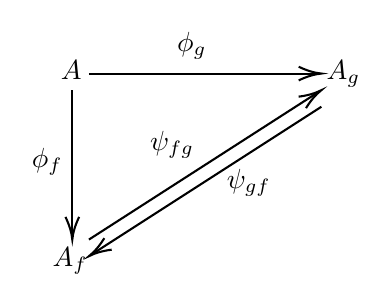
\begin{tikzpicture}[x=0.75pt,y=0.75pt,yscale=-1,xscale=1]
%uncomment if require: \path (0,476); %set diagram left start at 0, and has height of 476

%Straight Lines [id:da5476358885072219] 
\draw    (184,144) -- (294,144) ;
\draw [shift={(296,144)}, rotate = 180] [color={rgb, 255:red, 0; green, 0; blue, 0 }  ][line width=0.75]    (10.93,-3.29) .. controls (6.95,-1.4) and (3.31,-0.3) .. (0,0) .. controls (3.31,0.3) and (6.95,1.4) .. (10.93,3.29)   ;
%Straight Lines [id:da6784403518520925] 
\draw    (176,152) -- (176,222) ;
\draw [shift={(176,224)}, rotate = 270] [color={rgb, 255:red, 0; green, 0; blue, 0 }  ][line width=0.75]    (10.93,-3.29) .. controls (6.95,-1.4) and (3.31,-0.3) .. (0,0) .. controls (3.31,0.3) and (6.95,1.4) .. (10.93,3.29)   ;
%Straight Lines [id:da09322133204309413] 
\draw    (184,224) -- (294.32,153.08) ;
\draw [shift={(296,152)}, rotate = 147.26] [color={rgb, 255:red, 0; green, 0; blue, 0 }  ][line width=0.75]    (10.93,-3.29) .. controls (6.95,-1.4) and (3.31,-0.3) .. (0,0) .. controls (3.31,0.3) and (6.95,1.4) .. (10.93,3.29)   ;
%Straight Lines [id:da9376471110100983] 
\draw    (296,160) -- (185.68,230.92) ;
\draw [shift={(184,232)}, rotate = 327.26] [color={rgb, 255:red, 0; green, 0; blue, 0 }  ][line width=0.75]    (10.93,-3.29) .. controls (6.95,-1.4) and (3.31,-0.3) .. (0,0) .. controls (3.31,0.3) and (6.95,1.4) .. (10.93,3.29)   ;

% Text Node
\draw (169,136.4) node [anchor=north west][inner sep=0.75pt]    {$A$};
% Text Node
\draw (165,226.4) node [anchor=north west][inner sep=0.75pt]    {$A_{f}$};
% Text Node
\draw (297,136.4) node [anchor=north west][inner sep=0.75pt]    {$A_{g}$};
% Text Node
\draw (225,122.4) node [anchor=north west][inner sep=0.75pt]    {$\phi _{g}$};
% Text Node
\draw (155,178.4) node [anchor=north west][inner sep=0.75pt]    {$\phi _{f}$};
% Text Node
\draw (212,170.4) node [anchor=north west][inner sep=0.75pt]    {$\psi _{fg}$};
% Text Node
\draw (249,188.4) node [anchor=north west][inner sep=0.75pt]    {$\psi _{gf}$};


\end{tikzpicture}
\end{center}
Now it suffices to show $\psi_{fg}$ and $\psi_{gf}$ are identity maps. By the preceding discussion we have $\phi_f=\psi_{fg}\circ\psi_{gf}\circ\phi_f$. Then for any $s\in S_f$, we have $\psi_{fg}\circ\psi_{gf}\circ\phi_f(s)$ is a unit. Again by the universal property there exists a unique ring homomorphism $\varphi_f:A_f\to A_f$ such that $\psi_{fg}\circ\psi_{gf}\circ\phi_f=\varphi_f\circ\phi_f$.
\begin{center}


\tikzset{every picture/.style={line width=0.75pt}} %set default line width to 0.75pt        

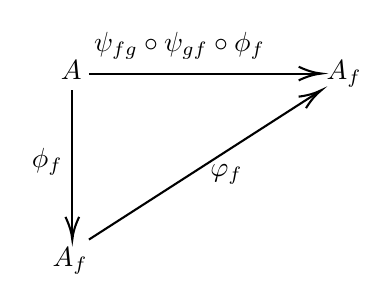
\begin{tikzpicture}[x=0.75pt,y=0.75pt,yscale=-1,xscale=1]
%uncomment if require: \path (0,476); %set diagram left start at 0, and has height of 476

%Straight Lines [id:da5476358885072219] 
\draw    (184,144) -- (294,144) ;
\draw [shift={(296,144)}, rotate = 180] [color={rgb, 255:red, 0; green, 0; blue, 0 }  ][line width=0.75]    (10.93,-3.29) .. controls (6.95,-1.4) and (3.31,-0.3) .. (0,0) .. controls (3.31,0.3) and (6.95,1.4) .. (10.93,3.29)   ;
%Straight Lines [id:da6784403518520925] 
\draw    (176,152) -- (176,222) ;
\draw [shift={(176,224)}, rotate = 270] [color={rgb, 255:red, 0; green, 0; blue, 0 }  ][line width=0.75]    (10.93,-3.29) .. controls (6.95,-1.4) and (3.31,-0.3) .. (0,0) .. controls (3.31,0.3) and (6.95,1.4) .. (10.93,3.29)   ;
%Straight Lines [id:da09322133204309413] 
\draw    (184,224) -- (294.32,153.08) ;
\draw [shift={(296,152)}, rotate = 147.26] [color={rgb, 255:red, 0; green, 0; blue, 0 }  ][line width=0.75]    (10.93,-3.29) .. controls (6.95,-1.4) and (3.31,-0.3) .. (0,0) .. controls (3.31,0.3) and (6.95,1.4) .. (10.93,3.29)   ;

% Text Node
\draw (169,136.4) node [anchor=north west][inner sep=0.75pt]    {$A$};
% Text Node
\draw (165,226.4) node [anchor=north west][inner sep=0.75pt]    {$A_{f}$};
% Text Node
\draw (297,136.4) node [anchor=north west][inner sep=0.75pt]    {$A_{f}$};
% Text Node
\draw (185,122.4) node [anchor=north west][inner sep=0.75pt]    {$\psi _{fg} \circ \psi _{gf} \circ \phi _{f}$};
% Text Node
\draw (155,178.4) node [anchor=north west][inner sep=0.75pt]    {$\phi _{f}$};
% Text Node
\draw (241,186.4) node [anchor=north west][inner sep=0.75pt]    {$\varphi _{f}$};


\end{tikzpicture}
\end{center}
Therefore by the unique property we have $\varphi_f=\psi_{fg}\circ\psi_{gf}$. Note $\varphi_f\circ\phi_f=\phi_f=1_f\circ\phi_f$, hence $\varphi_f=1_f$. Similarly we have $\varphi_g=1_g$, hence $\psi_{fg}\circ\psi_{gf}=1_f$, $\psi_{gf}\circ\psi_{fg}=1_g$, whence $A_f\cong A_g$.\par
(ii) We first show that there exists such $u$. Note that $X_g\subset X_f$, therefore 
$$
r\left( g \right) =\bigcap{\left\{ \mathfrak{p} \in \mathrm{Spec}\left( A \right) :g\subset \mathfrak{p} \right\}}\subset \bigcap{\left\{ \mathfrak{p} \in \mathrm{Spec}\left( A \right) :f\subset \mathfrak{p} \right\}}=r\left( f \right) ,
$$
hence there exists some $u$ such that $g^n=uf$. We use the universal property to define $\rho$. Consider the map $\phi_g:A\to A_g$. Note that $\phi_g(f)=f/1$ is a unit in $A_g$, hence by the universal property of the ring of fractions, there exists a unique $\rho:A_f\to A_g$ such that $\phi_g=\rho\circ\phi_f$.
\begin{center}


\tikzset{every picture/.style={line width=0.75pt}} %set default line width to 0.75pt        

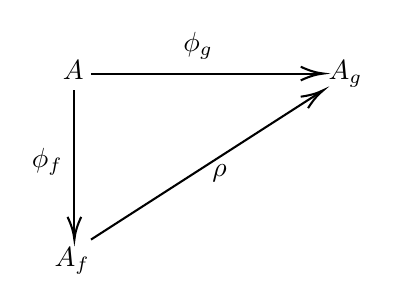
\begin{tikzpicture}[x=0.75pt,y=0.75pt,yscale=-1,xscale=1]
%uncomment if require: \path (0,476); %set diagram left start at 0, and has height of 476

%Straight Lines [id:da5476358885072219] 
\draw    (184,144) -- (294,144) ;
\draw [shift={(296,144)}, rotate = 180] [color={rgb, 255:red, 0; green, 0; blue, 0 }  ][line width=0.75]    (10.93,-3.29) .. controls (6.95,-1.4) and (3.31,-0.3) .. (0,0) .. controls (3.31,0.3) and (6.95,1.4) .. (10.93,3.29)   ;
%Straight Lines [id:da6784403518520925] 
\draw    (176,152) -- (176,222) ;
\draw [shift={(176,224)}, rotate = 270] [color={rgb, 255:red, 0; green, 0; blue, 0 }  ][line width=0.75]    (10.93,-3.29) .. controls (6.95,-1.4) and (3.31,-0.3) .. (0,0) .. controls (3.31,0.3) and (6.95,1.4) .. (10.93,3.29)   ;
%Straight Lines [id:da09322133204309413] 
\draw    (184,224) -- (294.32,153.08) ;
\draw [shift={(296,152)}, rotate = 147.26] [color={rgb, 255:red, 0; green, 0; blue, 0 }  ][line width=0.75]    (10.93,-3.29) .. controls (6.95,-1.4) and (3.31,-0.3) .. (0,0) .. controls (3.31,0.3) and (6.95,1.4) .. (10.93,3.29)   ;

% Text Node
\draw (169,136.4) node [anchor=north west][inner sep=0.75pt]    {$A$};
% Text Node
\draw (165,226.4) node [anchor=north west][inner sep=0.75pt]    {$A_{f}$};
% Text Node
\draw (297,136.4) node [anchor=north west][inner sep=0.75pt]    {$A_{g}$};
% Text Node
\draw (154,178.4) node [anchor=north west][inner sep=0.75pt]    {$\phi _{f}$};
% Text Node
\draw (241,186.4) node [anchor=north west][inner sep=0.75pt]    {$\rho $};
% Text Node
\draw (227,122.4) node [anchor=north west][inner sep=0.75pt]    {$\phi _{g}$};


\end{tikzpicture}
\end{center}
To show that $\rho$ is invariant of $f$ and $g$, it suffices to show the following diagram is commutative: 
\begin{center}


\tikzset{every picture/.style={line width=0.75pt}} %set default line width to 0.75pt        

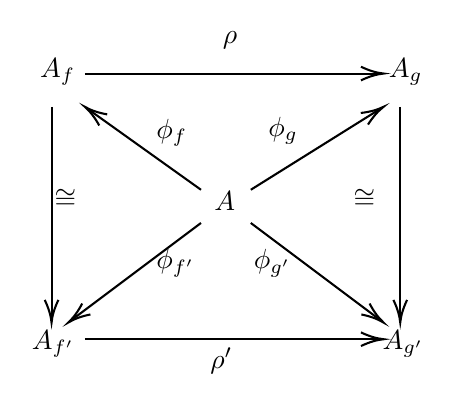
\begin{tikzpicture}[x=0.75pt,y=0.75pt,yscale=-1,xscale=1]
%uncomment if require: \path (0,476); %set diagram left start at 0, and has height of 476

%Straight Lines [id:da8717349823458596] 
\draw    (208,128) -- (350,128) ;
\draw [shift={(352,128)}, rotate = 180] [color={rgb, 255:red, 0; green, 0; blue, 0 }  ][line width=0.75]    (10.93,-3.29) .. controls (6.95,-1.4) and (3.31,-0.3) .. (0,0) .. controls (3.31,0.3) and (6.95,1.4) .. (10.93,3.29)   ;
%Straight Lines [id:da8101407119517832] 
\draw    (192,144) -- (192,246) ;
\draw [shift={(192,248)}, rotate = 270] [color={rgb, 255:red, 0; green, 0; blue, 0 }  ][line width=0.75]    (10.93,-3.29) .. controls (6.95,-1.4) and (3.31,-0.3) .. (0,0) .. controls (3.31,0.3) and (6.95,1.4) .. (10.93,3.29)   ;
%Straight Lines [id:da09196826456503504] 
\draw    (360,144) -- (360,246) ;
\draw [shift={(360,248)}, rotate = 270] [color={rgb, 255:red, 0; green, 0; blue, 0 }  ][line width=0.75]    (10.93,-3.29) .. controls (6.95,-1.4) and (3.31,-0.3) .. (0,0) .. controls (3.31,0.3) and (6.95,1.4) .. (10.93,3.29)   ;
%Straight Lines [id:da057945691531280374] 
\draw    (208,256) -- (350,256) ;
\draw [shift={(352,256)}, rotate = 180] [color={rgb, 255:red, 0; green, 0; blue, 0 }  ][line width=0.75]    (10.93,-3.29) .. controls (6.95,-1.4) and (3.31,-0.3) .. (0,0) .. controls (3.31,0.3) and (6.95,1.4) .. (10.93,3.29)   ;
%Straight Lines [id:da9625395466917612] 
\draw    (264,184) -- (209.63,145.16) ;
\draw [shift={(208,144)}, rotate = 35.54] [color={rgb, 255:red, 0; green, 0; blue, 0 }  ][line width=0.75]    (10.93,-3.29) .. controls (6.95,-1.4) and (3.31,-0.3) .. (0,0) .. controls (3.31,0.3) and (6.95,1.4) .. (10.93,3.29)   ;
%Straight Lines [id:da5510521034677156] 
\draw    (288,184) -- (350.3,145.06) ;
\draw [shift={(352,144)}, rotate = 147.99] [color={rgb, 255:red, 0; green, 0; blue, 0 }  ][line width=0.75]    (10.93,-3.29) .. controls (6.95,-1.4) and (3.31,-0.3) .. (0,0) .. controls (3.31,0.3) and (6.95,1.4) .. (10.93,3.29)   ;
%Straight Lines [id:da37678733813370746] 
\draw    (288,200) -- (350.4,246.8) ;
\draw [shift={(352,248)}, rotate = 216.87] [color={rgb, 255:red, 0; green, 0; blue, 0 }  ][line width=0.75]    (10.93,-3.29) .. controls (6.95,-1.4) and (3.31,-0.3) .. (0,0) .. controls (3.31,0.3) and (6.95,1.4) .. (10.93,3.29)   ;
%Straight Lines [id:da24163284759778492] 
\draw    (264,200) -- (201.6,246.8) ;
\draw [shift={(200,248)}, rotate = 323.13] [color={rgb, 255:red, 0; green, 0; blue, 0 }  ][line width=0.75]    (10.93,-3.29) .. controls (6.95,-1.4) and (3.31,-0.3) .. (0,0) .. controls (3.31,0.3) and (6.95,1.4) .. (10.93,3.29)   ;

% Text Node
\draw (185,119.4) node [anchor=north west][inner sep=0.75pt]    {$A_{f}$};
% Text Node
\draw (353,119.4) node [anchor=north west][inner sep=0.75pt]    {$A_{g}$};
% Text Node
\draw (181,250.4) node [anchor=north west][inner sep=0.75pt]    {$A_{f^{\prime }}$};
% Text Node
\draw (350,250.4) node [anchor=north west][inner sep=0.75pt]    {$A_{g^{\prime }}$};
% Text Node
\draw (269,183.4) node [anchor=north west][inner sep=0.75pt]    {$A$};
% Text Node
\draw (273,106.4) node [anchor=north west][inner sep=0.75pt]    {$\rho $};
% Text Node
\draw (267,258.4) node [anchor=north west][inner sep=0.75pt]    {$\rho ^{\prime }$};
% Text Node
\draw (241,148.4) node [anchor=north west][inner sep=0.75pt]    {$\phi _{f}$};
% Text Node
\draw (241,211.4) node [anchor=north west][inner sep=0.75pt]    {$\phi _{f^{\prime }}$};
% Text Node
\draw (288,211.4) node [anchor=north west][inner sep=0.75pt]    {$\phi _{g^{\prime }}$};
% Text Node
\draw (295,147.4) node [anchor=north west][inner sep=0.75pt]    {$\phi _{g}$};
% Text Node
\draw (192,182.4) node [anchor=north west][inner sep=0.75pt]    {$\cong $};
% Text Node
\draw (336,182.4) node [anchor=north west][inner sep=0.75pt]    {$\cong $};


\end{tikzpicture}
\end{center}
which is a direct verification and we omit the details.\par
(iii) By the universal property we have $\rho_1:A(U)\to A(U^\prime)$ such that $\phi_g=\rho_1\circ\phi_f$ and $\rho_2:A(U^\prime)\to A(U)$ such that $\phi_f=\rho_2\circ\phi_g$. Since $U$ and $U^\prime$ are identical, we have $\phi_g=\phi_f$ are epimorphisms. Therefore by the right cancellation we have $\rho_1$ and $\rho_2$ are both identity maps.\par
(iv) It is a straight-forward verification that the following diagram is commutative.
\begin{center}


\tikzset{every picture/.style={line width=0.75pt}} %set default line width to 0.75pt        

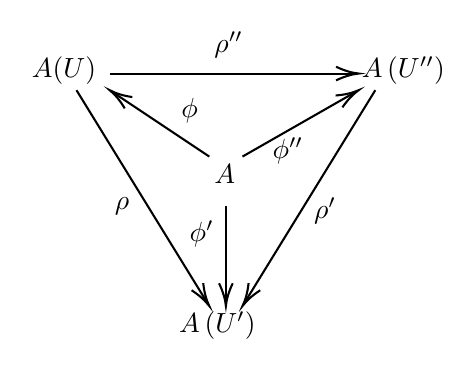
\begin{tikzpicture}[x=0.75pt,y=0.75pt,yscale=-1,xscale=1]
%uncomment if require: \path (0,476); %set diagram left start at 0, and has height of 476

%Straight Lines [id:da0007906455837118909] 
\draw    (168,152) -- (286,152) ;
\draw [shift={(288,152)}, rotate = 180] [color={rgb, 255:red, 0; green, 0; blue, 0 }  ][line width=0.75]    (10.93,-3.29) .. controls (6.95,-1.4) and (3.31,-0.3) .. (0,0) .. controls (3.31,0.3) and (6.95,1.4) .. (10.93,3.29)   ;
%Straight Lines [id:da03230323110404765] 
\draw    (152,160) -- (214.95,262.3) ;
\draw [shift={(216,264)}, rotate = 238.39] [color={rgb, 255:red, 0; green, 0; blue, 0 }  ][line width=0.75]    (10.93,-3.29) .. controls (6.95,-1.4) and (3.31,-0.3) .. (0,0) .. controls (3.31,0.3) and (6.95,1.4) .. (10.93,3.29)   ;
%Straight Lines [id:da15004016285227206] 
\draw    (296,160) -- (233.05,262.3) ;
\draw [shift={(232,264)}, rotate = 301.61] [color={rgb, 255:red, 0; green, 0; blue, 0 }  ][line width=0.75]    (10.93,-3.29) .. controls (6.95,-1.4) and (3.31,-0.3) .. (0,0) .. controls (3.31,0.3) and (6.95,1.4) .. (10.93,3.29)   ;
%Straight Lines [id:da8641523929893957] 
\draw    (216,192) -- (169.66,161.11) ;
\draw [shift={(168,160)}, rotate = 33.69] [color={rgb, 255:red, 0; green, 0; blue, 0 }  ][line width=0.75]    (10.93,-3.29) .. controls (6.95,-1.4) and (3.31,-0.3) .. (0,0) .. controls (3.31,0.3) and (6.95,1.4) .. (10.93,3.29)   ;
%Straight Lines [id:da9891349937389746] 
\draw    (232,192) -- (286.26,160.99) ;
\draw [shift={(288,160)}, rotate = 150.26] [color={rgb, 255:red, 0; green, 0; blue, 0 }  ][line width=0.75]    (10.93,-3.29) .. controls (6.95,-1.4) and (3.31,-0.3) .. (0,0) .. controls (3.31,0.3) and (6.95,1.4) .. (10.93,3.29)   ;
%Straight Lines [id:da7868530248532117] 
\draw    (224,216) -- (224,262) ;
\draw [shift={(224,264)}, rotate = 270] [color={rgb, 255:red, 0; green, 0; blue, 0 }  ][line width=0.75]    (10.93,-3.29) .. controls (6.95,-1.4) and (3.31,-0.3) .. (0,0) .. controls (3.31,0.3) and (6.95,1.4) .. (10.93,3.29)   ;

% Text Node
\draw (129,142.4) node [anchor=north west][inner sep=0.75pt]    {$A( U)$};
% Text Node
\draw (288,142.4) node [anchor=north west][inner sep=0.75pt]    {$A\left( U^{\prime \prime }\right)$};
% Text Node
\draw (200,265.4) node [anchor=north west][inner sep=0.75pt]    {$A\left( U^{\prime }\right)$};
% Text Node
\draw (217,194.4) node [anchor=north west][inner sep=0.75pt]    {$A$};
% Text Node
\draw (201,162.4) node [anchor=north west][inner sep=0.75pt]    {$\phi $};
% Text Node
\draw (205,221.4) node [anchor=north west][inner sep=0.75pt]    {$\phi ^{\prime }$};
% Text Node
\draw (245,181.4) node [anchor=north west][inner sep=0.75pt]    {$\phi ^{\prime \prime }$};
% Text Node
\draw (169,210.4) node [anchor=north west][inner sep=0.75pt]    {$\rho $};
% Text Node
\draw (265,210.4) node [anchor=north west][inner sep=0.75pt]    {$\rho ^{\prime }$};
% Text Node
\draw (217,130.4) node [anchor=north west][inner sep=0.75pt]    {$\rho ^{\prime \prime }$};


\end{tikzpicture}
\end{center}
which is routine by definition and we omit the details.\par
(v) We first show that the collection of all such $\{A(U_i)\}_{i\in I}$ is a direct system. To see this, partially order $\{A(U_i)\}_{i\in I}$ with inclusion, and consider the restriction homomorphism $\rho_{ij}:A(U_i)\to A(U_j)$. Now consider the following diagram: 
\begin{center}


\tikzset{every picture/.style={line width=0.75pt}} %set default line width to 0.75pt        

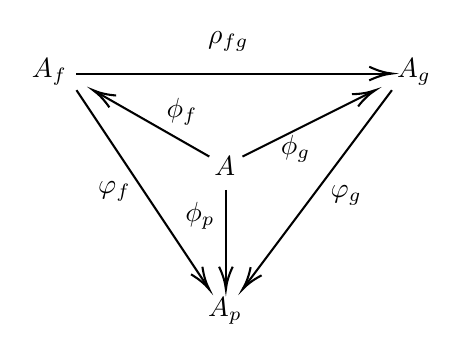
\begin{tikzpicture}[x=0.75pt,y=0.75pt,yscale=-1,xscale=1]
%uncomment if require: \path (0,476); %set diagram left start at 0, and has height of 476

%Straight Lines [id:da9569123890238775] 
\draw    (176,144) -- (326,144) ;
\draw [shift={(328,144)}, rotate = 180] [color={rgb, 255:red, 0; green, 0; blue, 0 }  ][line width=0.75]    (10.93,-3.29) .. controls (6.95,-1.4) and (3.31,-0.3) .. (0,0) .. controls (3.31,0.3) and (6.95,1.4) .. (10.93,3.29)   ;
%Straight Lines [id:da8983550294853244] 
\draw    (176,152) -- (238.89,246.34) ;
\draw [shift={(240,248)}, rotate = 236.31] [color={rgb, 255:red, 0; green, 0; blue, 0 }  ][line width=0.75]    (10.93,-3.29) .. controls (6.95,-1.4) and (3.31,-0.3) .. (0,0) .. controls (3.31,0.3) and (6.95,1.4) .. (10.93,3.29)   ;
%Straight Lines [id:da9806288407678148] 
\draw    (328,152) -- (257.2,246.4) ;
\draw [shift={(256,248)}, rotate = 306.87] [color={rgb, 255:red, 0; green, 0; blue, 0 }  ][line width=0.75]    (10.93,-3.29) .. controls (6.95,-1.4) and (3.31,-0.3) .. (0,0) .. controls (3.31,0.3) and (6.95,1.4) .. (10.93,3.29)   ;
%Straight Lines [id:da6344162334432626] 
\draw    (240,184) -- (185.74,152.99) ;
\draw [shift={(184,152)}, rotate = 29.74] [color={rgb, 255:red, 0; green, 0; blue, 0 }  ][line width=0.75]    (10.93,-3.29) .. controls (6.95,-1.4) and (3.31,-0.3) .. (0,0) .. controls (3.31,0.3) and (6.95,1.4) .. (10.93,3.29)   ;
%Straight Lines [id:da784764619977564] 
\draw    (256,184) -- (318.21,152.89) ;
\draw [shift={(320,152)}, rotate = 153.43] [color={rgb, 255:red, 0; green, 0; blue, 0 }  ][line width=0.75]    (10.93,-3.29) .. controls (6.95,-1.4) and (3.31,-0.3) .. (0,0) .. controls (3.31,0.3) and (6.95,1.4) .. (10.93,3.29)   ;
%Straight Lines [id:da1271306957260394] 
\draw    (248,200) -- (248,246) ;
\draw [shift={(248,248)}, rotate = 270] [color={rgb, 255:red, 0; green, 0; blue, 0 }  ][line width=0.75]    (10.93,-3.29) .. controls (6.95,-1.4) and (3.31,-0.3) .. (0,0) .. controls (3.31,0.3) and (6.95,1.4) .. (10.93,3.29)   ;

% Text Node
\draw (153,135.4) node [anchor=north west][inner sep=0.75pt]    {$A_{f}$};
% Text Node
\draw (329,135.4) node [anchor=north west][inner sep=0.75pt]    {$A_{g}$};
% Text Node
\draw (238,250.4) node [anchor=north west][inner sep=0.75pt]    {$A_{\mathfrak{p}}$};
% Text Node
\draw (241,182.4) node [anchor=north west][inner sep=0.75pt]    {$A$};
% Text Node
\draw (238,122.4) node [anchor=north west][inner sep=0.75pt]    {$\rho _{fg}$};
% Text Node
\draw (185,194.4) node [anchor=north west][inner sep=0.75pt]    {$\varphi _{f}$};
% Text Node
\draw (297,196.4) node [anchor=north west][inner sep=0.75pt]    {$\varphi _{g}$};
% Text Node
\draw (218,154.4) node [anchor=north west][inner sep=0.75pt]    {$\phi _{f}$};
% Text Node
\draw (227,204.4) node [anchor=north west][inner sep=0.75pt]    {$\phi _{\mathfrak{p}}$};
% Text Node
\draw (273,172.4) node [anchor=north west][inner sep=0.75pt]    {$\phi _{g}$};


\end{tikzpicture}
\end{center}
whence we have $\varphi_f=\varphi_g\circ\rho_{fg}$ and hence by the universal property of direct limit we have a homomorphism $\varphi:\varinjlim A(U_i)\to A_\mathfrak{p}$, as shown in the following diagram: 
\begin{center}


\tikzset{every picture/.style={line width=0.75pt}} %set default line width to 0.75pt        

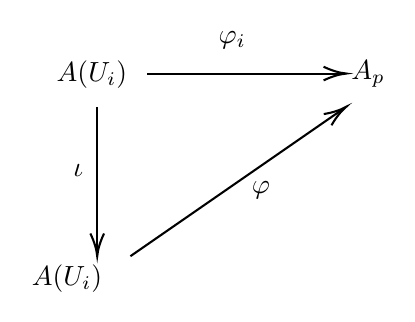
\begin{tikzpicture}[x=0.75pt,y=0.75pt,yscale=-1,xscale=1]
%uncomment if require: \path (0,476); %set diagram left start at 0, and has height of 476

%Straight Lines [id:da09848593079462153] 
\draw    (176,160) -- (176,230) ;
\draw [shift={(176,232)}, rotate = 270] [color={rgb, 255:red, 0; green, 0; blue, 0 }  ][line width=0.75]    (10.93,-3.29) .. controls (6.95,-1.4) and (3.31,-0.3) .. (0,0) .. controls (3.31,0.3) and (6.95,1.4) .. (10.93,3.29)   ;
%Straight Lines [id:da2207608618263297] 
\draw    (200,144) -- (294,144) ;
\draw [shift={(296,144)}, rotate = 180] [color={rgb, 255:red, 0; green, 0; blue, 0 }  ][line width=0.75]    (10.93,-3.29) .. controls (6.95,-1.4) and (3.31,-0.3) .. (0,0) .. controls (3.31,0.3) and (6.95,1.4) .. (10.93,3.29)   ;
%Straight Lines [id:da4274016983494544] 
\draw    (192,232) -- (294.36,161.14) ;
\draw [shift={(296,160)}, rotate = 145.3] [color={rgb, 255:red, 0; green, 0; blue, 0 }  ][line width=0.75]    (10.93,-3.29) .. controls (6.95,-1.4) and (3.31,-0.3) .. (0,0) .. controls (3.31,0.3) and (6.95,1.4) .. (10.93,3.29)   ;

% Text Node
\draw (155,136.4) node [anchor=north west][inner sep=0.75pt]    {$A( U_{i})$};
% Text Node
\draw (297,136.4) node [anchor=north west][inner sep=0.75pt]    {$A_{\mathfrak{p}}$};
% Text Node
\draw (143,234.4) node [anchor=north west][inner sep=0.75pt]    {$\varinjlim A( U_{i})$};
% Text Node
\draw (233,122.4) node [anchor=north west][inner sep=0.75pt]    {$\varphi _{i}$};
% Text Node
\draw (249,194.4) node [anchor=north west][inner sep=0.75pt]    {$\varphi $};
% Text Node
\draw (163,186.4) node [anchor=north west][inner sep=0.75pt]    {$\iota $};


\end{tikzpicture}
\end{center}
now it suffices to show that $\varphi$ is an isomorphism. First we show that $\varphi$ is injective. To do this, suppose $b\in\mathrm{Ker}\varphi$, then $\varphi(b)=0$. Write $b=\rho_f(a/f^k)$, then 
$$
0=\varphi(b)=\varphi\circ\rho_f(a/f^k)=\varphi_f(a/f^k).
$$
Note that $\varphi_f(a/f^k)=a/f^k$, hence $a/f^k=0/1\in A_\mathfrak{p}$. Therefore there exists some $s\in S$ such that $sa=0$. Then 
$$
\rho _f\left( a/f^n \right) =\rho _{sf}\circ \rho _{sf,f}\left( a/f^n \right) =\rho _f\left( as^n/\left( sf \right) ^n \right) =\rho _f\left( 0/1 \right) =0.
$$
Therefore $b=0$ and hence $\varphi$ is injective. To show $\varphi$ is surjective, pick $a/s\in A_\mathfrak{p}$, then $a/s\in A_s$, hence $\rho_s(a/s)\in\varinjlim A(U_i)$, therefore $\varphi\circ\rho_s(a/s)=\varphi_s(a/s)=a/s$, which finished the proof.
\end{proof}
\begin{problem}\em
Show that the presheaf of Exercise 8.23 has the following property. Let $(U_i)_{i\in I}$ be a covering of $X$ by basic open sets. For each $i\in I$ let $s_i\in A(U_i)$ be such that, for each pair of indices $i$, $j$, the images of $s_i$ and $s_j$ in $A(U_i\cap U_j)$ are equal. Then there exists a unique $s\in A$($=A(X)$) whose image in $A(U_i)$ is $s_i$, for all $i\in I$.\par
This essentially implies that the presheaf is a \textbf{sheaf}.
\end{problem}